
\documentclass[11pt]{article}
\usepackage[T1]{fontenc}
\usepackage[margin=0.82in]{geometry}
\usepackage{amsmath,amssymb,amsthm,mathtools}
\usepackage{booktabs,tabularx,array,longtable}
\usepackage{graphicx}
\usepackage{microtype}
\usepackage{flafter}
\usepackage{float}
\usepackage{tikz-cd}
\usepackage{enumitem}
\usepackage{xcolor}
\usepackage[font=small,labelfont=bf]{caption}
\usepackage{hyperref}
\hypersetup{
  colorlinks=true,
  linkcolor=blue!55!black,
  citecolor=blue!55!black,
  urlcolor=blue!55!black,
  pdftitle={Kolmogorov Structure Functions, Inverse-Colimits, and Cofibrations: Solving ARC-AGI-3 with Compute-Bounded Self-Improving Agents},
  pdfauthor={Alexander Kolpakov},
  pdfkeywords={ARC-AGI-3, Kolmogorov structure function, free energy, inverse colimit, cofibration, PowerPlay, artificial curiosity, self-improving agent}
}

\newtheorem{theorem}{Theorem}
\newtheorem{proposition}[theorem]{Proposition}
\newtheorem{corollary}[theorem]{Corollary}
\newtheorem{lemma}[theorem]{Lemma}
\theoremstyle{definition}
\newtheorem{definition}[theorem]{Definition}
\newtheorem{assumption}[theorem]{Assumption}
\theoremstyle{remark}
\newtheorem{remark}[theorem]{Remark}

\newcommand{\F}{\mathcal{F}}
\newcommand{\Comp}{\operatorname{Comp}}
\newcommand{\Risk}{\operatorname{Risk}}
\newcommand{\Syn}{\mathsf{Syn}_{\Sigma}}
\newcommand{\Art}{\mathsf{Art}}
\newcommand{\Pol}{\mathsf{Pol}}
\newcommand{\Beh}{\mathsf{Beh}}
\newcommand{\Cert}{\mathsf{Cert}}
\newcommand{\Sem}[1]{\mathopen{[\![}#1\mathclose{]\!]}}
\newcommand{\Lan}{\operatorname{Lan}}
\newcommand{\colimv}{\operatorname*{colim}}
\newcommand{\limv}{\operatorname*{lim}}
\newcommand{\E}{\mathbb{E}}
\newcommand{\Prb}{\mathbb{P}}
\newcommand{\Pos}[1]{[#1]_{+}}
\newcommand{\RepoURL}{https://github.com/sashakolpakov/gkm}

\title{Kolmogorov Structure Functions, Inverse-Colimits, and Cofibrations: Solving ARC-AGI-3 with Compute-Bounded Self-Improving Agents}

\author{Alexander Kolpakov\footnote{corresponding author; e-mail address: kolpakov.alexander@gmail.com; postal address: University of Austin, 522~Congress Street, Austin TX, 78701 USA}}
\date{August 2026}

\begin{document}
\maketitle
\raggedbottom

\begin{abstract}
We present the G\"odel--Kolmogorov Machine (GKM), a replay-gated program-growth
architecture for interactive ARC-AGI-3. A coding language model proposes
game- and level-dependent executable components, while fixed host code admits a
candidate only after fresh execution and independent path replay. We represent
retained solver growth as a sequence of pushout attachments, relate candidate
selection to Kolmogorov structure functions and free-energy duality, and connect
the resulting loop to G\"odel machines, PowerPlay, and artificial curiosity.
Under explicit finiteness and fair-search or stagewise full-support assumptions,
we prove compute-completeness for deterministic games with finite winning
traces. A frozen 25-game campaign verifies 181 of 183 levels
($98.9071\%$ raw coverage; $98.1166\%$ in Competition Mode), and exact
source histories exhibit retained-leg reuse together with nonmonotone marginal
description growth. GKM is a universal producer of verified executable solvers;
its learned outputs remain game- and level-dependent rather than constituting a
single fixed runtime policy.
\end{abstract}

\textbf{Keywords:} G\"odel--Kolmogorov Machine; ARC-AGI-3; Kolmogorov
structure function; free energy; inverse colimit; cofibration; PowerPlay; artificial
curiosity; self-improving coding agent; program synthesis.

\section{Introduction}
ARC-AGI-3 is an interactive benchmark for fluid agentic intelligence. Its environments
withhold the object vocabulary, action semantics, mechanics, and goal; a solver must
acquire these through interaction and then act efficiently~\cite{chollet2019measure,arcagi3}.
This format exposes a central distinction that endpoint accuracy alone hides. Two agents
may reach the same level while one repeatedly reconstructs a disposable plan and the
other extends a retained executable theory. The latter is the phenomenon studied here:
program growth under verification, compression pressure, and a finite compute budget.

The G\"odel--Kolmogorov Machine treats a solver not as a single final program but as a
verified construction history
\[
  X_0\xhookrightarrow{j_1}P_1\simeq_{T_1}X_1
     \xhookrightarrow{j_2}P_2\simeq_{T_2}\cdots
     \xhookrightarrow{j_k}P_k\simeq_{T_k}X_k,
\]
together with the proposed legs, bindings, source deltas, action paths, and replay
certificates that created each stage. The coding model is not merely asked to emit the
next action. It proposes a new component and the morphisms by which that component is
attached to the incumbent program. The harness evaluates the resulting cocone,
executes it from a fresh reset, and promotes it only after the recorded full path
independently replays to the new depth. That deeper path re-establishes all earlier
depth obligations by truncation, although it need not coincide with the historically
stored paths for those depths. In this sense the category-theoretic language is
architectural: the objects are executable components, the morphisms are bindings and
interface maps, and the inverse-colimit apex is the linked program that actually runs.

We use \emph{solving ARC-AGI-3} in a compute-indexed sense. At any finite budget $B$,
the archive exposes a verified frontier $V_B$. Because promotions are retained,
$V_B$ is monotone in $B$. More strongly, the proposal language contains literal finite
action programs as well as reusable legs. Consequently every deterministic game with a
finite winning trace has a finite representative in the search space. A fair universal
search therefore reaches it after finite computation; an LLM proposer satisfying the
stagewise full-support condition below reaches it almost surely as compute grows.
Practical models determine the waiting-time distribution, but not the underlying
existence result. The empirical campaign reports where one such search process stopped
at a predeclared solver-budget floor, not an assertion that the frontier is a fixed
capacity ceiling.

The G\"odel--Kolmogorov Machine sits directly in the lineage of Schmidhuber's G\"odel machine,
PowerPlay, and artificial curiosity. The G\"odel machine supplies the idea that a
self-rewrite must cross a verification gate~\cite{schmidhuber2007godel}. PowerPlay
supplies continual acquisition of the simplest still-unsolved task while preserving old
skills~\cite{schmidhuber2013powerplay}. Artificial curiosity supplies intrinsic reward
for learning or compression progress~\cite{schmidhuber2010curiosity}. The
G\"odel--Kolmogorov Machine replaces a formal utility proof by an executable replay
certificate, instantiates PowerPlay on the
externally ordered but hidden ARC levels, and evaluates structural progress through the
free energy dual of a Kolmogorov structure function.

The paper makes five contributions.
\begin{enumerate}[leftmargin=2.1em]
\item It defines an \emph{inverse-colimit attachment} in which an LLM proposes a new
leg, its interface, a cofibration, and an attaching map. The linked candidate is the
corresponding pushout; strictly additive acquisitions form a sequential colimit, while
validated debriefs move within replay-equivalence classes.
\item It places the implemented source statistic inside the computable-proxy
loss--complexity theory, deriving the structure function, Legendre--Fenchel free energy,
partition function, susceptibility, and complexity ratchet.
\item It gives a compute-completeness theorem for finite replay-verifiable games, with
deterministic universal-search and stagewise full-support forms.
\item It makes the PowerPlay and artificial-curiosity correspondence operational:
replay preserves the task archive, free energy orders candidate extensions, and expected
frontier reduction values informative probes.
\item It reports a frozen 25-game release spanning 181 of 183 levels, two complete
uniform chronological histories, and solved-checkpoint comparisons whose reuse claims
require both a source-level factorization and replay.
\end{enumerate}

For concision in the remainder of the paper, we abbreviate the
G\"odel--Kolmogorov Machine as \emph{GKM}.

\section{Architectural Lineage: G\"odel Machines, PowerPlay, and Artificial Curiosity}
\subsection{From proof-gated self-rewrite to replay-gated program growth}
A G\"odel machine may rewrite any part of itself after its proof searcher establishes
that the rewrite improves expected utility under the machine's formal axioms and
resource model~\cite{schmidhuber2007godel}. GKM keeps the decisive architectural move---
self-revision under a gate---while changing the certificate. ARC environments provide a
terminating empirical judge for finite claims: reset, execute, record, reset again, and
replay. A promotion is therefore admitted by a behavioral proof object consisting of
source identity, checkpoint identity, an action path, reached depth, environment
version, and replay result. The gate is weaker than a theorem about all future states,
but stronger than the proposer's own assertion that its code worked.

The split is deliberate. The proposer is generative and fallible; the verifier is fixed
and adversarial to the proposal. A proposed attachment can be arbitrarily ambitious,
including a new perception system, search procedure, literal plan, or refactor. Its
admission obligation is narrow and executable: it must extend the validated task set and
must not invalidate the retained replay archive. This division lets an LLM supply
mathematical construction data without granting it authority over the truth of the
construction.

\subsection{GKM as an external-task PowerPlay}
PowerPlay repeatedly searches for a pair consisting of a task not solved by the current
solver and a solver modification that solves the new task while preserving all prior
skills; its search order favors pairs that are compact and quickly validated
\cite{schmidhuber2013powerplay}. ARC-AGI-3 supplies an externally generated curriculum:
the next exposed level is the currently selected unsolved task, while the search for a
small attachment and the optional debrief recover PowerPlay's simplicity pressure and
its ``wow effect'' of compressing or accelerating old solutions.

\begin{table}[H]
\centering
\small
\begin{tabularx}{\textwidth}{@{}>{\raggedright\arraybackslash}p{0.25\textwidth}>{\raggedright\arraybackslash}X>{\raggedright\arraybackslash}X@{}}
\toprule
PowerPlay object & GKM realization & Executable certificate \\
\midrule
Current problem solver & Promoted library, players, dispatcher, and checkpoint & Clean source snapshot plus checkpoint hash \\
Simplest still-unsolved task & Next unreproduced ARC level, failed reuse obligation, or compression task & Failure of incumbent composition or a shorter replay-equivalent candidate \\
Solver modification & LLM-supplied leg, boundary, binding, and residual glue & Source diff and reconstructed inverse-colimit attachment diagram \\
Correctness demonstration & Fresh candidate execution plus independent replay of its full path & Reached depth, stored path, and replay status \\
No forgetting & A depth-$k$ path reaches every earlier depth & Canonical first-passage truncations of the validated path \\
Simplicity pressure & $R+\lambda\Comp$ and marginal source action & free energy comparison and source ledger \\
\bottomrule
\end{tabularx}
\caption{The GKM loop as a concrete, externally tasked PowerPlay instance.}
\label{tab:powerplay-correspondence}
\end{table}

The analogy is structural rather than rhetorical. PowerPlay's task solver pair is the
atomic search object; GKM's atomic object is the task--attachment pair
$(T_k,D_k)$, where $D_k$ is the inverse diagram whose colimit extends the incumbent.
The retained archive prevents catastrophic forgetting at the artifact level, and the
complexity coordinate biases the search toward reuse or small glue when existing legs
already span the new task.

\subsection{Artificial curiosity as free energy progress}
Artificial curiosity rewards improvement of a predictor or compressor rather than raw
unpredictability. Interesting observations are those that are initially surprising but
become compressible with attainable learning effort~\cite{schmidhuber2010curiosity}.
Let $\mathcal H_t$ be the current archive of candidate mechanics, goals, or solver
presentations after history $h_t$, and define the archive free energy envelope
\begin{equation}
  \Phi_t(\lambda)=\inf_{q\in\mathcal H_t}
       \bigl(L_t(q)+\lambda\Comp(q)\bigr).
  \label{eq:curiosity-envelope}
\end{equation}
For a candidate probe $a$ and possible observation $o$, a one-step intrinsic value is
\begin{equation}
  I_t(a)=\E_{o\sim \widehat P_t(\cdot\mid a)}
   \Pos{\Phi_t(\lambda)-\Phi_{t+1}^{(a,o)}(\lambda)}.
  \label{eq:curiosity-progress}
\end{equation}
This is compression progress expressed on the entire loss--complexity frontier. Archive
disagreement is a computable approximation: probe where surviving hypotheses predict
different frame deltas, goal atoms, or action outcomes, provided the disagreement is
neither trivial nor apparently impossible. The repository's open-ended program uses
this decomposition---disagreement, learning progress, partial solvability, triviality,
and impossibility---to identify tasks near the competence frontier~\cite{gkmrepo}.

External reward and curiosity are complementary. Sparse level completion supplies the
PowerPlay task boundary; Eq.~\eqref{eq:curiosity-progress} allocates interactions inside
that boundary. The resulting loop is
\[
\begin{aligned}
  \text{probe for compressible novelty}
   &\longrightarrow \text{propose a cofibrant attachment}\\
   &\longrightarrow \text{execute and replay}
    \longrightarrow \text{retain or refactor}.
\end{aligned}
\]

\section{Kolmogorov Structure Functions and free energy Duality}
\subsection{A computable complexity coordinate}
For finite data $x$, Kolmogorov's structure function is
\begin{equation}
  h_x(\alpha)=\min\{\log |S|:x\in S,\ K(S)\leq\alpha\},
  \label{eq:classical-structure-function}
\end{equation}
which separates model description from residual data description
\cite{kolmogorov1965,solomonoff1964,vereshchagin2004,live2008}. The useful object for an
interactive solver is the inverse parameterization: the minimum executable complexity
needed to attain a behavioral risk.

Fix a computable representation and accounting rule $\kappa$. For a retained artifact
$s$, let
\[
  D_\kappa(s)=\Comp_\kappa(s)\in\mathbb R_{\ge 0}
\]
be its computed description energy. In the implementation, $\kappa$ counts nonblank,
noncomment source lines and AST container-literal elements in the retained leg and
player files. This coordinate is representation-dependent, as every computable coding
coordinate must be, but its role in the mathematics is exact: recent work formulates
model structure functions for computable complexity coordinates and proves their
free energy/Legendre--Fenchel duality~\cite{losscomplexity}. Accordingly $D_\kappa$ is
not an informal stand-in appended after the argument. It is the operational coordinate
on which the dual theory is evaluated: universal-machine complexity supplies the ideal
coordinate up to the invariance theorem, while $\kappa$ supplies an executable chart in
which artifacts can be measured, selected, and falsified.

Let $m$ be the number of levels in a game, $V(s)$ the depth reproduced by fresh replay,
and $R(s)=m-V(s)$. For an auditable proposal set $\mathcal P$, define
\begin{equation}
  C^{*}_{\mathcal P,\kappa}(r)
  =\inf\{D_\kappa(s):s\in\mathcal P,\ R(s)\le r\}.
  \label{eq:model-function}
\end{equation}
Equivalently, in the level coordinate,
\begin{equation}
  \widehat C_{\mathcal P,\kappa}(v)
  =\inf\{D_\kappa(s):s\in\mathcal P,\ V(s)\ge v\}
  =C^{*}_{\mathcal P,\kappa}(m-v).
  \label{eq:structure-function}
\end{equation}
The complete promoted history supplies measured points in this landscape and therefore
upper bounds on the finite-sample frontier. A debrief can move downward at fixed $R$ by
replacing a literal program with a shorter factorization; a new mechanic moves leftward
by reducing $R$, usually at a positive complexity cost.

\subsection{Legendre--Fenchel free energy}
The zero-temperature free energy envelope is
\begin{align}
  \Phi_{\mathcal P,\kappa}(\lambda)
   &=\inf_{s\in\mathcal P}\bigl(R(s)+\lambda D_\kappa(s)\bigr) \\
   &=\inf_r\bigl(r+\lambda C^{*}_{\mathcal P,\kappa}(r)\bigr),
  \qquad \lambda>0.
  \label{eq:model-dual}
\end{align}
Its Legendre--Fenchel reconstruction is
\begin{equation}
  \underline C_{\mathcal P,\kappa}(r)
  =\sup_{\lambda>0}\frac{\Phi_{\mathcal P,\kappa}(\lambda)-r}{\lambda}
  \le C^{*}_{\mathcal P,\kappa}(r),
  \label{eq:model-biconjugate}
\end{equation}
with equality at supported points of the lower convex envelope. If the minimizer
$s_\lambda$ is unique and locally stable, the envelope theorem yields
\begin{equation}
  \Phi'_{\mathcal P,\kappa}(\lambda)=D_\kappa(s_\lambda),
  \qquad
  R(s_\lambda)=\Phi_{\mathcal P,\kappa}(\lambda)
          -\lambda\Phi'_{\mathcal P,\kappa}(\lambda).
  \label{eq:model-envelope}
\end{equation}
Thus kinks in $\Phi$ are changes of selected program regime, while the full structure
function retains unsupported but scientifically meaningful artifacts.

For finite $\mathcal P$, introduce inverse temperature $\beta$ and
\begin{align}
  Z_{\beta,\lambda}
    &=\sum_{s\in\mathcal P}
       \exp\{-\beta(R(s)+\lambda D_\kappa(s))\}, \\
  \F_{\beta,\lambda}
    &=-\beta^{-1}\log Z_{\beta,\lambda}.
  \label{eq:partition-free energy}
\end{align}
Then
\begin{equation}
  \lim_{\beta\to\infty}\F_{\beta,\lambda}
  =\Phi_{\mathcal P,\kappa}(\lambda).
  \label{eq:zero-temperature}
\end{equation}
The thermodynamic derivatives are exact:
\begin{equation}
  \frac{\partial \F_{\beta,\lambda}}{\partial\lambda}
    =\E_{\beta,\lambda}[D_\kappa(s)],
  \qquad
  \frac{\partial^2 \F_{\beta,\lambda}}{\partial\lambda^2}
    =-\beta\,\operatorname{Var}_{\beta,\lambda}[D_\kappa(s)].
  \label{eq:free energy-derivatives}
\end{equation}
Accordingly a nonnegative complexity susceptibility is
\begin{equation}
  \chi_C(\beta,\lambda)
     =\beta\,\operatorname{Var}_{\beta,\lambda}[D_\kappa(s)]
     =-\frac{\partial^2 \F_{\beta,\lambda}}{\partial\lambda^2},
  \label{eq:susceptibility}
\end{equation}
up to the conventional placement of the factor $\beta$. Peaks identify parameter
regions in which small changes in parsimony pressure exchange qualitatively different
solver structures. This is the mathematically grounded reason to sweep $\lambda$ rather
than report one regularized optimum.

\subsection{The complexity ratchet and historical action}
For two candidates $s$ and $s'$, the more complex candidate is selected exactly when
its risk reduction purchases its additional description:
\begin{equation}
  R(s)-R(s')>\lambda\bigl(D_\kappa(s')-D_\kappa(s)\bigr).
  \label{eq:complexity-ratchet}
\end{equation}
This is the complexity ratchet. It prevents open-ended growth from degenerating into
unpriced accumulation: each cell must buy new control, prediction, transfer, or a
shorter solution elsewhere.

The retained state coordinate $D_\kappa(s_k)$ and the historical construction action
are distinct. For shared-library source $\ell_k$ and player source $p_k$, define
\begin{equation}
  C_k=\Pos{d(\ell_k)-d(\ell_{k-1})}
      +\Pos{d(p_k)-d(p_{k-1})},
  \qquad
  C_{\le k}=\sum_{j\le k}C_j.
  \label{eq:marginal-c}
\end{equation}
The path-dependent free energy is
\begin{equation}
  \F^{\mathrm{hist}}_\lambda(s_k)
    =R(s_k)+\lambda C_{\le k}.
  \label{eq:historical-free energy}
\end{equation}
It records the price paid along a lineage even when a later refactor compresses the
retained endpoint.

\begin{proposition}[Positive-variation decomposition]
For any real sequence $x_0,\ldots,x_n$,
\begin{equation}
  \sum_{k=1}^{n}\Pos{x_k-x_{k-1}}
  =x_n-x_0+\sum_{k=1}^{n}\Pos{x_{k-1}-x_k}.
  \label{eq:positive-variation}
\end{equation}
Consequently the historical GKM charge equals endpoint growth plus the amount of
measured description later removed, summed separately over the charged files.
\end{proposition}
\begin{proof}
Use $u=\Pos{u}-\Pos{-u}$ for every increment $u=x_k-x_{k-1}$ and telescope.
\end{proof}

This identity makes the two coordinates complementary rather than competing. The
structure function asks how short the best retained representative is at a risk level;
the historical action asks how much positive construction was traversed to reach it.

\section{Inverse-Colimit Program Growth and Cofibrant Attachments}
\label{sec:category}
\subsection{Finite program presentations grounded in source}
Fix a typed signature $\Sigma$ with node sorts for definitions, formal parameters,
state predicates, call sites, action literals, control edges, and dispatcher bindings.
Let $\Syn$ be the category of finite $\Sigma$-typed incidence graphs and type-preserving
graph morphisms. Typed graphs form a presheaf-style adhesive category: pushouts along
monomorphisms are well behaved, and the finite presentations used here are closed under
the finite pushouts below~\cite{maclane1998,riehl2016category,lack2005adhesive}.

A promoted Python snapshot $s$ determines a finite presentation
$\Gamma(s)\in\Syn$ by its definitions, signatures, call graph, control dependencies,
and dispatch bindings. This is a mathematical extraction from the source, not a claim
that the current harness materializes a generic category-theory object at runtime. The
repository stores Python files; source, AST, call-site, and diff audits are the ground
truth from which the relevant objects and arrows are reconstructed.

We designate monomorphisms in $\Syn$ as \emph{cofibrations}. A cofibration preserves an
embedded interface literally while permitting new nodes and edges to be attached around
it. Identities and composites are cofibrations, and pushout of a cofibration is again a
cofibration, as in a Waldhausen-style category~\cite{waldhausen1985}. This is precisely
the persistence property needed by a growing leg library. It does not imply that every
Python edit is a monomorphism: an acquisition edge may be cofibrational, whereas a
debrief that rewrites already admitted source is represented separately by validated
replay equivalence.

\subsection{Inverse diagrams and the LLM-supplied cell}
A finite category $J$ is \emph{inverse} when its objects admit a degree function such
that every nonidentity morphism strictly lowers degree. Let $\mathbb V$ be the inverse
span category with objects $\partial,0,1$, degrees
$\deg(\partial)=1$, $\deg(0)=\deg(1)=0$, and arrows
$\partial\to0$, $\partial\to1$.

\begin{definition}[LLM-supplied inverse-colimit attachment]
Given an incumbent artifact $X_{k-1}\in\Syn$, the proposer emits source embodying
\begin{enumerate}[leftmargin=2em]
\item a boundary or interface object $A_k$;
\item a new executable leg or cell $B_k$;
\item a cofibration $i_k:A_k\hookrightarrow B_k$; and
\item an attaching/binding morphism $a_k:A_k\to X_{k-1}$.
\end{enumerate}
These data define an inverse diagram $D_k:\mathbb V\to\Syn$,
\[
  X_{k-1}\xleftarrow{a_k}A_k\xrightarrow{i_k}B_k.
\]
Its \emph{inverse colimit}---the colimit of this inverse-shaped diagram---is the linked
candidate
\begin{equation}
  P_k=\colimv_{\mathbb V}D_k
     \cong X_{k-1}\sqcup_{A_k}B_k.
  \label{eq:inverse-colimit-attachment}
\end{equation}
\end{definition}

The word \emph{inverse} modifies the indexing shape, not the universal construction:
interface arrows run from the higher-degree overlap toward the lower-degree incumbent
and proposed cell, while the universal object is a colimit. Operationally, $A_k$ is the
formal dependency surface of the new code, $a_k$ binds that surface to definitions and
state relations already present, and $i_k$ includes the same surface into the proposed
cell. The LLM therefore contributes both objects and morphisms; a lattice of observed
state--action pairs cannot encode these invented interfaces or bindings.

% Standalone source: figure_sources/inverse_colimit_attachment_standalone.tex
\begin{figure}[H]
\centering
\begin{tikzcd}[column sep=huge,row sep=large]
A_k \arrow[r,hook,"i_k"] \arrow[d,"a_k"']
  & B_k \arrow[d,"b_k"] \\
X_{k-1} \arrow[r,hook,"j_k"']
  & P_k=X_{k-1}\sqcup_{A_k}B_k
\end{tikzcd}
\caption{The inverse-colimit cell attachment. The proposer supplies $B_k$, $A_k$,
$i_k$, and $a_k$; the universal cocone supplies $j_k$ and $b_k$. Cobase change forces
$j_k$ to be a cofibration. The other cocone map $b_k$ need not be monic unless further
hypotheses are imposed on $a_k$.}
\label{fig:inverse-colimit-pushout}
\end{figure}

\begin{theorem}[Cofibrant persistence and universal gluing]
If $i_k:A_k\hookrightarrow B_k$ is a cofibration and cofibrations in $\Syn$ are stable
under cobase change, then the incumbent map
$j_k:X_{k-1}\hookrightarrow P_k$ in Fig.~\ref{fig:inverse-colimit-pushout} is a
cofibration. For every artifact $Y$ and compatible pair
$f:X_{k-1}\to Y$, $g:B_k\to Y$ satisfying
$f\circ a_k=g\circ i_k$, there is a unique $u:P_k\to Y$ with
$u\circ j_k=f$ and $u\circ b_k=g$.
\end{theorem}
\begin{proof}
The first statement is stability of cofibrations under pushout along $a_k$; the second
is the universal property of the pushout.
\end{proof}

The theorem is the exact content of persistent reuse at the presentation level. The
incumbent program survives in the candidate through $j_k$; new executable structure
enters through $b_k$; and the attaching map records how open slots are bound. A thin
level player can therefore have small conditional description even when it invokes a
large leg whose definition was paid for at an earlier stage.

There is also a semantic obligation. On compilable presentations and a finite validation
suite $T$, let
\[
  \Sem{-}_T:\mathsf{Syn}_{\Sigma,T}\longrightarrow\Beh(E)
\]
map source presentations and auditable call/binding morphisms to their replay-observed
transition presentations. Applying this functor to the source cocone induces a canonical
comparison morphism
\begin{equation}
  \theta_{k,T}:\colimv\!\bigl(
    \Sem{X_{k-1}}_T
      \xleftarrow{}\Sem{A_k}_T
      \xrightarrow{}\Sem{B_k}_T\bigr)
  \longrightarrow \Sem{P_k}_T.
  \label{eq:semantic-comparison}
\end{equation}
If $\theta_{k,T}$ is an isomorphism, the source pushout is also the behavioral pushout on
$T$ and is universal among compatible observed-behavior cocones. The implementation does
not assume global colimit preservation. Source-level call tracing checks the intended
factorization, while fresh execution and replay test the finite semantic comparison at
the admitted histories. Thus the category theory supplies the construction obligation
and the verifier decides whether its executable realization is behaviorally valid.

\subsection{Many-leg inverse colimits}
A proposal may bind several incumbent legs, introduce several cells, and identify
higher-order overlaps among them. Let $J_k$ be a finite inverse category with one
distinguished incumbent object, positive-degree interface/overlap objects, and
degree-zero cell objects. For a cell $c$, define its boundary object by
\begin{equation}
  \partial_cD_k=
  \colimv_{(j\to c),\,\deg(j)>0}D_k(j),
  \label{eq:cell-boundary}
\end{equation}
with the canonical map $\partial_cD_k\to D_k(c)$. We call the presentation
\emph{cellularly cofibrant} when each such boundary map for a newly proposed cell is a
cofibration.

\begin{proposition}[Iterated inverse-colimit attachment]
Suppose the new degree-zero cells admit an ordering in which the boundary of each cell
maps into the incumbent together with cells attached earlier in the order. Then
$\colimv_{J_k}D_k$ is computed by a finite sequence of pushouts along the boundary
cofibrations in Eq.~\eqref{eq:cell-boundary}. The composite map from the incumbent into
the resulting apex is a cofibration.
\end{proposition}
\begin{proof}
Attach the ordered cells one at a time. At each stage the boundary has a map into the
partial apex by hypothesis, so the next apex is a pushout. Pushout stability makes the
partial-apex inclusion a cofibration; closure under composition gives the final claim.
\end{proof}

This is the many-leg version of Fig.~\ref{fig:inverse-colimit-pushout}. The proposer
constructs a finite inverse presentation---existing definitions, new cells, overlaps,
and bindings---and the linked solver is its universal gluing. The repository does not
call a generic colimit routine; Python name resolution and execution realize the cocone,
while the categorical presentation states what structure that source embodies.

\subsection{Acquisition, debrief, and replay equivalence}
The raw linked candidate need not be the final promoted text. A debrief may inline,
extract, rename, or parameterize code after the new competence has been found. For a
finite validation suite $T$, write
\begin{equation}
  P\simeq_T Q
  \label{eq:replay-equivalence}
\end{equation}
when both artifacts compile and their independently replayed certificates agree on the
obligations in $T$. A promotion therefore has the source-level factorization
\begin{equation}
  X_{k-1}\xhookrightarrow{\;j_k\;}P_k
  \;\simeq_{T_k}\;X_k,
  \label{eq:cofibration-refactor-factorization}
\end{equation}
where the first arrow is the inverse-colimit acquisition and the second relation is an
optional replay-equivalent normalization. If no debrief intervenes, $X_k=P_k$.

Equation~\eqref{eq:cofibration-refactor-factorization} prevents two opposite mistakes.
A behavior-only inclusion does not exhibit the LLM-supplied cell and attaching map; a
raw source diff does not automatically prove a cofibration when incumbent code was
rewritten. The cofibration claim is made at the source level when unchanged interfaces,
definitions, and call sites witness the factorization. Replay equivalence then permits
semantic-preserving refactors without pretending that they are acquisitions of new
behavior.

When every stage is strictly additive, the candidates form a cofibration filtration
\begin{equation}
  X_0\xhookrightarrow{}X_1\xhookrightarrow{}\cdots
       \xhookrightarrow{}X_k,
  \qquad X_\infty=\colimv_kX_k.
  \label{eq:sequential-colimit}
\end{equation}
With debriefs, the preserved history is instead the zigzag of
Eq.~\eqref{eq:cofibration-refactor-factorization}: acquisitions are colimit attachments
and refactors move within validated equivalence classes. The WIP and promoted snapshots
are therefore mathematically relevant provenance, not incidental logging.

For a set $L_k$ of available shared legs and player/binding code $g_i$, an ideal
two-part code is
\begin{equation}
  D_{\mathrm{cone}}(k)
  =\sum_{\ell\in L_k}D(\ell)
   +\sum_{i=1}^{k}D(g_i\mid L_i)+O(\log k),
  \label{eq:cone-code}
\end{equation}
and the new-level marginal is
\begin{equation}
  \Delta D_{\mathrm{cone}}(k)
  =\sum_{\ell\in L_k\setminus L_{k-1}}D(\ell)
   +D(g_k\mid L_k)+O(\log k).
  \label{eq:cone-marginal}
\end{equation}
An old leg is paid for once; subsequent applications pay for the attaching morphism and
residual glue. This is the categorical content of the marginal-complexity troughs.

\subsection{Replay certificates as an inverse system}
The implementation validates reached depth, not identity with every earlier action
trace. Let $\Cert_j(E)$ be the set of finite replay certificates whose stored path,
executed from a fresh reset of environment $E$, reaches at least depth $j$. For a
certificate $c=(\pi,\eta)\in\Cert_k(E)$ with $k\ge j$, let
\begin{equation}
  \rho_{k,j}(c)
  \label{eq:certificate-restriction}
\end{equation}
truncate $\pi$ at its first passage to depth $j$ and retain the relevant source,
checkpoint, and environment metadata $\eta$. Then
\begin{equation}
  \rho_{j,i}\circ\rho_{k,j}=\rho_{k,i},
  \qquad i\le j\le k,
  \label{eq:certificate-coherence}
\end{equation}
so the depth certificates form an inverse system.

A replay-validated full path $c_k\in\Cert_k(E)$ determines the coherent family
\begin{equation}
  \bigl(\rho_{k,j}(c_k)\bigr)_{j\le k}
  \in\limv_{j\le k}\Cert_j(E).
  \label{eq:inverse-replay-limit}
\end{equation}
This is the exact no-forgetting statement implemented by a deeper full-path replay: it
re-establishes every shallower task. It does \emph{not} assert that
$\rho_{k,j}(c_k)$ equals the historical checkpoint path $c_j$; later solvers may reach
the same depth by a different route. Program acquisition and verification consequently
run in complementary directions: source grows by colimits of inverse-shaped attachment
diagrams, while a successful deep certificate restricts contravariantly to the earlier
depth obligations.

\begin{definition}[Replay-certified cofibrant attachment]
A proposed level-$k$ extension is replay-certified when
\begin{enumerate}[leftmargin=2em]
\item its source admits the factorization
$X_{k-1}\hookrightarrow P_k=X_{k-1}\sqcup_{A_k}B_k$ with
$A_k\hookrightarrow B_k$ a source-auditable cofibration;
\item the linked candidate compiles and fresh execution produces a finite path $\pi_k$;
\item an independent replay of $\pi_k$ reaches the required depth; and
\item the first-passage truncations of $\pi_k$ define the coherent family in
Eq.~\eqref{eq:inverse-replay-limit}.
\end{enumerate}
A source-level reuse certificate additionally identifies the unchanged incumbent
definition and the call or binding through which the new player factors.
\end{definition}

The definition gives the LLM the creative role the architecture requires without
confusing proposal with proof. It supplies the cell, boundary, and morphisms. The fixed
verifier decides whether their linked realization enters the archive.

\subsection{Few-shot transfer as a pointwise Kan extension}
Let $\Beh(E)$ be the category of finite typed transition-system presentations over the
action--observation signature induced by environment $E$, with label-preserving graph
morphisms. Replay-observed behaviors are finite objects of this presheaf-style category,
which has the finite colimits used below. Let $\mathcal L_k$ be the category of known leg
schemas and binding morphisms, and let
$K_k:\mathcal L_k\hookrightarrow\mathcal T_k$ include them into a category containing a
new task object $\tau$. A behavior functor $F_k:\mathcal L_k\to\Beh(E)$ extends to the
new task by the pointwise left Kan extension
\begin{equation}
  (\Lan_{K_k}F_k)(\tau)
  \cong \colimv_{(K_k\downarrow\tau)}F_k\circ\pi,
  \label{eq:kan-extension}
\end{equation}
whenever the indicated colimit exists~\cite{maclane1998,riehl2016category}. The comma
category consists of known legs together with admissible ways of binding them into the
new task. The emitted player source is read as a finite subdiagram of this comma
category: it selects incumbent legs, invents missing bindings, and adds a residual cell
when the frozen library is insufficient. This is a formal semantics of the source-level
construction; the runtime need not invoke a general Kan-extension implementation.

Equation~\eqref{eq:kan-extension} explains why the morphism vocabulary is the inductive
bias. A missing object predicate, color slot, transition interface, or binding cannot be
recovered by the colimit operation alone; the proposer must enrich the category. Once
the correct morphisms are present, reuse is obtained by universal gluing rather than by
learning an unrelated action sequence.

\section{Compute-Bounded Solving and Asymptotic Completion}
\label{sec:compute}
\subsection{The budget-indexed frontier}
Let $\mathcal A_B$ be the archive of replay-validated artifacts obtainable with total
proposal-and-verification budget at most $B$, and define
\begin{equation}
  V_B(g)=\max_{s\in\mathcal A_B}V_g(s).
  \label{eq:budget-frontier}
\end{equation}
Because the archive retains promoted artifacts, $B\le B'$ implies
$\mathcal A_B\subseteq\mathcal A_{B'}$ and therefore $V_B(g)\le V_{B'}(g)$. This is the
basic sense in which an incomplete endpoint is compute-bounded: it is a point on a
monotone search trajectory, not a negative result about the existence of a continuation.

\subsection{Finite attachment completeness}
Consider a game with $m$ levels and suppose there exists a finite chain of replay-valid
attachments that completes it. Equivalently for the existence argument, suppose there
is one finite full-game action program. Literal action programs are admissible cells, so
abstraction is not required for completeness; it is required to make the waiting time
scientifically and practically tolerable.

\begin{assumption}[Fair dovetailed proposal and recognizable success]
Finite attachment presentations are effectively enumerable. Deterministic search
fairly dovetails candidate index with execution time and action budget, so every finite
candidate is eventually run for every finite resource bound. In the stochastic version,
once depth $k$ has been reached, each proposal trial has conditional probability at
least $p_k>0$ of emitting a replay-valid continuation to depth $k+1$. A successful
finite replay is recognized and promoted.
\end{assumption}

\begin{theorem}[Compute completeness]
Under the preceding assumption, some complete replay-valid artifact is found after
finite computation by fair deterministic dovetailing. In the stochastic version, let
$\tau_k$ be the number of proposal trials required to advance from depth $k$ to $k+1$.
Then
\begin{equation}
  \Prb(\tau_k>n)\le(1-p_k)^n,
  \qquad
  \E[\tau_k]\le p_k^{-1},
  \label{eq:geometric-stage}
\end{equation}
and for any integers $n_0,\ldots,n_{m-1}\ge0$,
\begin{equation}
  \Prb\!\left(\sum_{k=0}^{m-1}\tau_k>
                    \sum_{k=0}^{m-1}n_k\right)
  \le\sum_{k=0}^{m-1}(1-p_k)^{n_k}.
  \label{eq:completion-tail}
\end{equation}
Consequently the probability that the game remains incomplete converges to zero as the
number of proposal trials allocated to every reached stage tends to infinity, and
\begin{equation}
  \E\!\left[\sum_{k=0}^{m-1}\tau_k\right]
  \le\sum_{k=0}^{m-1}p_k^{-1}.
  \label{eq:completion-expectation}
\end{equation}
\end{theorem}
\begin{proof}
The finite winning presentation has a finite enumeration index and succeeds within
some finite execution and action bound. Fair dovetailing eventually reaches that triple
and the recognizer promotes it. In the stochastic case, conditional
failure for $n$ trials is at most $(1-p_k)^n$, giving
Eq.~\eqref{eq:geometric-stage}. If every $\tau_k\le n_k$, their sum is at most
$\sum n_k$; the union bound gives Eq.~\eqref{eq:completion-tail}. The expectation bound
follows by summing the geometric bounds. No independence between stages is required
beyond the stated conditional lower bounds.
\end{proof}

\begin{corollary}[Finite-trace bound]\label{cor:finite-trace}
Let a deterministic resettable game have $q<\infty$ available actions and a winning path
of length $L<\infty$. Breadth-first enumeration of action strings finds a winning path
after testing at most
\begin{equation}
  1+q+q^2+\cdots+q^L=
  \begin{cases}
    (q^{L+1}-1)/(q-1), & q>1,\\
    L+1, & q=1
  \end{cases}
  \label{eq:finite-trace-bound}
\end{equation}
candidates. Hence every finitely solvable deterministic replay-verifiable game is solved
with finite compute.
\end{corollary}

\begin{corollary}[Compute-indexed solution of a finite ARC suite]
Let $\mathcal G$ be a finite suite of deterministic, resettable ARC games. If every
$g\in\mathcal G$ has a finite full-game winning trace over a finite action alphabet,
then a fair GKM scheduler with literal-trace fallback completes every game after finite
computation. If $q_g$ is the action-alphabet size and $L_g$ the length of one winning
trace, a separate breadth-first schedule tests no more than
\begin{equation}
  \sum_{g\in\mathcal G}\sum_{\ell=0}^{L_g}q_g^\ell
  \label{eq:finite-suite-bound}
\end{equation}
trace candidates before all such witnesses have been encountered.
\end{corollary}
\begin{proof}
Apply Corollary~\ref{cor:finite-trace} game by game and sum the finite bounds. The
search need not know the values $L_g$ in advance.
\end{proof}

\begin{corollary}[Universal-search fallback]
If the scheduler interleaves the LLM with fair dovetailed enumeration of finite programs,
every finite replay-valid solver program is eventually found. The LLM, inherited legs,
and free energy ordering reshape the waiting-time distribution; they are not needed for
the bare existence guarantee. This is the resource-sensitive universality principle
behind universal sequential search~\cite{levin1973}.
\end{corollary}

The theorem and corollaries are the formal content of the paper's compute claim. The
claim is not that a finite practical budget is sufficient for every game. It is that
finite solvability plus an enumerable language and recognizable replay imply finite
search completion, and that stagewise lower-bounded full-support proposal converges to
the same result with probability one. Category-theoretic reuse, PowerPlay retention, curiosity, and
free energy selection are what turn this otherwise astronomical guarantee into an
architecture for reducing the waiting time.

\subsection{Open-endedness beyond a fixed game set}
A fixed finite benchmark eventually saturates. Open-ended growth requires an endogenous
ecology
\begin{equation}
  \mathcal E_{t+1}=G(\mathcal E_t,\mathcal A_t,\mathcal H_t)
  \label{eq:ecology}
\end{equation}
that generates tasks near the archive's competence frontier. PowerPlay supplies the
continual task solver loop; artificial curiosity supplies a value for experiments that
produce learning progress; free energy prevents complexity from increasing without
payoff; and inverse-colimit attachments preserve the reusable program structure. The
forward research program is therefore not merely to spend more compute on a closed list,
but to couple compute to an archive-driven sequence of solvable, nontrivial, structurally
novel tasks.

\section{GKM Implementation and Repository-Grounded Protocol}
\label{sec:implementation}
\subsection{Code-level correspondence}
The public repository separates the conceptual roles used above. Its ARC laboratory
contains modules named \texttt{gkm\_legs.py}, \texttt{llm\_binder.py},
\texttt{cofibrant.py}, \texttt{powerplay.py}, and \texttt{replay\_scorecard.py},
alongside per-game promoted artifacts and tests~\cite{gkmrepo}. The exact names are not the mathematics, but they make the intended decomposition
inspectable. The table states the source-level interpretation used by the paper; the
repository remains the ground truth, and no claim is made that these modules instantiate
a general categorical runtime.

\begin{table}[H]
\centering
\small
\begin{tabularx}{\textwidth}{@{}>{\raggedright\arraybackslash}p{0.27\textwidth}>{\raggedright\arraybackslash}X>{\raggedright\arraybackslash}X@{}}
\toprule
Mathematical role & Executable realization & Retained evidence \\
\midrule
Cell $B_k$ & Shared leg or newly synthesized routine & Definition in a promoted \texttt{legs.py} snapshot \\
Boundary $A_k$ & Typed parameters, state predicate, expected pre/postcondition, or shared subroutine interface & Function signature and boundary checks \\
Attaching map $a_k$ & Level-specific argument binding, dispatch, sequencing, or call site & Winning player and source diff \\
Cofibration $i_k$ & Literal inclusion of the interface into the new leg presentation & Unchanged interface plus added body \\
Inverse-colimit apex $P_k$ & Library, players, and dispatcher compiled as one linked candidate & Candidate workspace and successful execution \\
Promoted artifact $X_k$ & $P_k$ itself or a replay-equivalent debrief & Clean promoted workspace and replay certificate \\
Inverse replay family & First-passage truncations of each checkpoint's full path & Checkpoint records, local segmentation, and replay status \\
PowerPlay archive & Ordered clean promotions and WIP provenance & Git history, sidecars, and run summaries \\
\bottomrule
\end{tabularx}
\caption{Correspondence between the formal construction and the repository artifact
surface.}
\label{tab:code-correspondence}
\end{table}

The scorecard implementation loads
\texttt{agent\_solutions/<game>\_legs/checkpoint.json}, splits the stored
\texttt{final\_path} into level segments by local replay, then replays those segments
against the remote ARC toolkit without invoking discovery or an LLM. It compares the
remote depth with the locally validated checkpoint and reports desynchronization as a
failure. Thus endpoint replay and proposer search are distinct computations.

\subsection{Interface and proposer}
The game-independent local interface exposes only
\begin{center}
\texttt{reset()}$\to$\emph{frame}, \quad
\texttt{step(action)}$\to$\emph{frame}, \quad
\texttt{frame()} \text{ (raw $64\times64$ grid)}, \\
\texttt{levels\_completed}, \quad \texttt{actions}, \quad
\texttt{terminal()}, \quad \texttt{clone()}.
\end{center}
No interface field names objects, mechanics, or goals. The proposer nevertheless carries
broad priors from pretraining and from the prompt: persistent objects, barriers,
controllable and autonomous entities, sparse reward, and the value of active probes. It
works in a disposable directory seeded from the highest clean promotion, may execute
cloned environments, and writes a \texttt{solve(env)} program.

For persistent frontiers, the active campaign also introduced an independent
observation-only side expert. This was a role escalation, not an
\texttt{ultra}-effort setting: the exploratory implementation reassigned an in-session
audit subagent whose model/effort field was not exposed. The expert received a private
copy of the exact parent and admitted clean same-frontier WIP, pursued a question
deliberately distinct from the live proposer, and experimented only through the public
Arena interface. It shared the host process/filesystem boundary, so its workspace was
taint-checked at every Arena launch and it could write only to the private copy.
Findings returned through the session were hypotheses, not promotions. Any path, patch,
or abstraction derived from them still required exact-parent provenance, a clean taint
verdict, and fresh replay before admission to the solver lineage.

The planned contiguous replication makes that tactic scheduler-controlled and
game-independent. After medium, high, xhigh, and the first max turn all end as clean
no-progress at one exact frontier, otherwise-idle capacity may run one independent
side expert (\(n=5\)); failure of the subsequent max reset/continuation pair permits
two distinct complexity assignments (\(n\geq7\)). Assignment classes are mechanism induction, state
representation, exact planning, and prefix compression, never game names or remembered
solutions. The scheduler allocates auxiliary capacity but does not author a
game-specific brief: each assignment must bind an authenticated same-frontier
\texttt{NATIVE\_SIDECAR\_REQUEST} emitted by the native proposer or a request
inside an admitted supervisory handoff. Manual, scheduler-authored, stale,
cross-frontier, and substituted requests are rejected. The contiguous role uses a minimal container input manifest, a separately
pinned model/effort, journaled usage, and quarantine-only output. These prospective
controls must not be read backward as properties of the exploratory sidecars.
At the same complexity-gated stage, the contiguous design may schedule a distinct
supervisory proposer. It receives only an immutable, hash-bound allowlist of the exact
frontier, the exact-parent and selected admitted-WIP solver-source snapshots, cited
native-proposer observations, and admitted side-expert evidence. Its
schema-validated \texttt{SUPERVISORY\_HANDOFF} must state the unresolved obligation,
cite the observations on which each hypothesis depends, propose bounded falsification
tests, record rejected alternatives and caveats, and include a Socratic challenge to
its own recommendation. It may include a typed same-frontier sidecar request, but that
request does not allocate capacity and remains subject to the deterministic scheduler.
The role cannot choose the game, effort, concurrency, WIP
policy, or promotion, and cannot mutate a solver. Its output remains quarantined until
the native proposer reproduces every cited source observation through the public
interface and the host verifier admits the resulting candidate by ordinary replay. At
most one such role is active per
frontier; a later round requires newly admitted evidence or a complete scheduler-defined
reset/continuation pair, rather than a retry-count increment alone. Thus the deterministic
scheduler,
native proposer, side expert, supervisory proposer, and host verifier have separate
receipt-bound authorities; every winning boundary must disclose whether its acquisition
attempt was exposed to an admitted supervisory handoff.
The clean retry count is the single operational complexity coordinate for both
medium-to-max effort escalation and max-plus-sidecar role escalation. It measures
repeated failure of stronger searches at an unchanged verified boundary; it is not
presented as an estimator of Kolmogorov complexity.

The harness treats proposer output as untrusted. Recognized private-runtime and hidden-
source access is blocked before execution, and tainted workspaces are rejected before
replay or promotion. Earlier attempts to access a private \texttt{env.\_game} object are
preserved as dirty WIP and excluded from all reported artifacts. The boundary is an
implemented path and lexical detector, not an information-flow theorem; the central
point is that prompt compliance is not used as the verification gate.

\subsection{Promotion as inverse-colimit construction}
The promoted workspace separates reusable and level-specific source.
\texttt{legs.py} contains shared components, \texttt{players.py} contains thin level
entry points, and \texttt{solve.py} dispatches by observed progress. Operationally, the
orchestrator first asks the proposer to compose incumbent legs and permits new source
when that attempt fails; mathematically, the emitted calls and bindings are the finite
comma diagram described in Section~\ref{sec:category}. The code does not invoke a generic
colimit library. The candidate is compiled and executed from reset, its full action path
is recorded, and that path is replayed independently from a second reset. A debrief may
then factor repeated glue into a higher-order leg, after which execution and replay are
repeated.

The operational cycle is:
\begin{enumerate}[leftmargin=2.1em]
\item seed from the highest clean artifact;
\item attempt a Kan-extension-style composition from incumbent legs;
\item propose missing objects and morphisms when the existing comma diagram is
insufficient;
\item compile the inverse colimit and execute it;
\item replay the full candidate path from a fresh reset; its first-passage
truncations re-certify all earlier depths, without requiring the earlier paths to be
identical;
\item measure the retained state and historical action, promote, and archive the
provenance;
\item optionally refactor inside the same replay-equivalence class.
\end{enumerate}
Known failed compositions are keyed by level and library hash, so a restart need not
repeat the same expensive search. A proposer-mutated checkpoint remains an untrusted
path candidate until the harness reproduces it.

\subsection{Implemented description coordinate}
For a source file $f$, $d(f)$ is the number of nonblank, noncomment lines plus the
number of elements in Python list, tuple, set, and dictionary literals found by AST
parsing. The literal term prevents a long action program written on one line from
receiving unit cost. If $\ell_k$ and $p_k$ are the library and player sources after
level $k$, the implementation computes Eq.~\eqref{eq:marginal-c}; the retained state
coordinate is
\begin{equation}
  D_k=d(\ell_k)+d(p_k).
  \label{eq:retained-description}
\end{equation}
This is the chosen computable $D_\kappa$ for the ARC artifacts. It omits comments,
identifier length, the fixed dispatcher, temporary probes, model inference, and
environment interactions. Those are separate compute coordinates rather than reasons to
remove the source coordinate from the theory. The correct scientific response is to
report the coding rule, compare artifacts under the same $\kappa$, and eventually sweep
multiple representations.

A small $C_k$ is a candidate sign of reuse, not a sufficient certificate. Reuse is
claimed only when the winning entry point directly invokes an unchanged earlier
component and the composite passes replay. This couples the scalar free energy trace to
the cofibration and attaching morphism visible in source.

\subsection{Artifact scope and reproduction}
The frozen release reports one canonical promoted artifact for each of the 25 public
games and reaches 181 of 183 levels; only \texttt{lf52} levels~9--10 remain outside
the claimed prefix. \texttt{wa30} and \texttt{ls20} additionally have complete
manuscript-level uniform construction histories. The artifact campaign is not a
repeated-seed estimate. It is a chronological observation of one compute-bounded growth
process, with exact endpoint replay and source provenance.
Universality is at the producer level: the same proposer contract, Arena surface,
blank scaffold, complexity coordinate, and replay gate generate every artifact. The
learned output is necessarily game- and level-dependent solver code; specialization of
that output is not a different architecture.

Three repository commands address different layers:
\begin{verbatim}
python arc/manuscript/build_artifact_history.py --check
ENDPOINT_ROOT=/path/to/arc_agi3_gkm_v2_181/artifacts \
ACQUISITION_ROOT=/path/to/arc_agi3_gkm_v2_181/acquisition_source \
RELEASE_RECEIPT=/path/to/arc_agi3_gkm_v2_181/receipts/\
140e37ca7014d5aa6a48a3808fd94e90209c56499dbcd7df9f0fe733a29a7681.json \
  make -C arc/manuscript reproduce
python arc/crack_lab/replay_scorecard.py --mode online --games all \
  --artifact-root arc/crack_lab/releases/arc_agi3_gkm_v2_181/artifacts \
  --release-receipt arc/crack_lab/releases/arc_agi3_gkm_v2_181/receipts/\
140e37ca7014d5aa6a48a3808fd94e90209c56499dbcd7df9f0fe733a29a7681.json \
  --expected-claimed-levels 181
\end{verbatim}
The history builder checks the two immutable uniform sidecars. The unified reproduction
entry point uses normalized capsules for endpoint certification, frozen acquisition
programs for $D(s)$ and marginal-complexity outputs, and source-history revision
\texttt{4d0e42f34d7b1db8305f03d725528dfdefe22511} for the source/reuse audit.
It invokes the receipt-bound historical release gate to revalidate the complete sealed
evidence chain. The online
scorecard repeats that gate before binding and locally segmenting the exact loaded
checkpoint bytes, then replays their stored paths against the public remote environments
with zero LLM tokens. Exact regeneration of stochastic proposal transcripts is a
different experiment from reproduction of the promoted solver.

\subsection{Numerical reconciliation}
Related score and accounting quantities are separated throughout this revision.
\begin{table}[H]
\centering
\small
\begin{tabularx}{\textwidth}{@{}p{0.36\textwidth}rX@{}}
\toprule
Quantity & Value & Meaning \\
\midrule
Official Competition-Mode score & $98.1166403783\%$ & Public all-game score over 25 games \\
Frozen-release raw coverage & $181/183=98.9071038251\%$ & Unweighted verified level fraction \\
Frozen-release stored/API actions & $7001/7069$ & Immutable paths / official scorecard calls \\
\texttt{wa30} uniform publication ledger & 318 & Nine fresh sequential promotion boundaries \\
\texttt{ls20} uniform publication ledger & 760 & Seven fresh sequential promotion boundaries \\
\bottomrule
\end{tabularx}
\caption{Distinct score and accounting quantities for the frozen v2 release. The
official ARC score and raw level fraction use different aggregations. The 68-call gap
between stored paths and the scorecard comprises 25 initial resets and 43 calls from a
transient \texttt{vc33} connection-reset recovery.}
\label{tab:numerical-reconciliation}
\end{table}

\section{Empirical Results}
The reported endpoints are reproduced from promoted checkpoints and action paths;
source-level interpretations below are confined to the 174 checkpoints admitted by the
pinned winning-source audit. The definitive replay-only Competition-Mode scorecard reports an official
all-game score of $98.11664037825032\%$ over all 25 public games. Its frozen raw
coverage is $181/183=98.907103825137\%$; the stored paths contain 7001 actions and the
scorecard records 7069 API calls. Neither quantity measures the larger clone-enabled
interaction and model-inference cost of discovery.

% Generated by scripts/generate_empirical_tables.py; do not edit.
\begin{table}[p]
\centering
\scriptsize
\setlength{\tabcolsep}{2.7pt}
\resizebox{\textwidth}{!}{%
\begin{tabular}{@{}lrrrrrrrrrrrrrr@{}}
\toprule
Game & Depth & Path & $D(s)$ & L1 & L2 & L3 & L4 & L5 & L6 & L7 & L8 & L9 & L10 & $C_{\leq k}$ \\
\midrule
\texttt{ar25} & 8/8 & 269 & 67 & 9 & 4 & 9 & 7 & 7 & 10 & 10 & 10 & $\mathrm{n/a}$ & $\mathrm{n/a}$ & 66 \\
\texttt{bp35} & 9/9 & 393 & 1280 & 210 & 174 & 108 & 102 & 44 & 128 & 174 & 79 & 260 & $\mathrm{n/a}$ & 1279 \\
\texttt{cd82} & 6/6 & 91 & 174 & 11 & 12 & 41 & 35 & 37 & 37 & $\mathrm{n/a}$ & $\mathrm{n/a}$ & $\mathrm{n/a}$ & $\mathrm{n/a}$ & 173 \\
\texttt{cn04} & 6/6 & 210 & 96 & 12 & 12 & 32 & 13 & 13 & 13 & $\mathrm{n/a}$ & $\mathrm{n/a}$ & $\mathrm{n/a}$ & $\mathrm{n/a}$ & 95 \\
\texttt{dc22} & 6/6 & 540 & 851 & 49 & 71 & 96 & 107 & 2 & 325 & $\mathrm{n/a}$ & $\mathrm{n/a}$ & $\mathrm{n/a}$ & $\mathrm{n/a}$ & 650 \\
\texttt{ft09} & 6/6 & 80 & 602 & 107 & 2 & 184 & 132 & 177 & 2 & $\mathrm{n/a}$ & $\mathrm{n/a}$ & $\mathrm{n/a}$ & $\mathrm{n/a}$ & 604 \\
\texttt{g50t} & 7/7 & 361 & 673 & 244 & 100 & 2 & 2 & 134 & 88 & 102 & $\mathrm{n/a}$ & $\mathrm{n/a}$ & $\mathrm{n/a}$ & 672 \\
\texttt{ka59} & 7/7 & 342 & 159 & 26 & 25 & 13 & 20 & 4 & 21 & 49 & $\mathrm{n/a}$ & $\mathrm{n/a}$ & $\mathrm{n/a}$ & 158 \\
\texttt{lf52} & 8/10 & 544 & 1419 & 116 & 119 & 2 & 217 & 96 & 352 & 307 & 209 & pending & pending & 1418 \\
\texttt{lp85} & 8/8 & 93 & 49 & 10 & 5 & 5 & 3 & 6 & 8 & 6 & 5 & $\mathrm{n/a}$ & $\mathrm{n/a}$ & 48 \\
\texttt{ls20} & 7/7 & 365 & 761 & 40 & 54 & 86 & 114 & 138 & 170 & 158 & $\mathrm{n/a}$ & $\mathrm{n/a}$ & $\mathrm{n/a}$ & 760 \\
\texttt{m0r0} & 6/6 & 230 & 358 & 24 & 29 & 159 & 27 & 46 & 72 & $\mathrm{n/a}$ & $\mathrm{n/a}$ & $\mathrm{n/a}$ & $\mathrm{n/a}$ & 357 \\
\texttt{r11l} & 6/6 & 115 & 1384 & 103 & 449 & 30 & 341 & 362 & 98 & $\mathrm{n/a}$ & $\mathrm{n/a}$ & $\mathrm{n/a}$ & $\mathrm{n/a}$ & 1383 \\
\texttt{re86} & 8/8 & 600 & 1873 & 105 & 133 & 237 & 343 & 343 & 176 & 297 & 238 & $\mathrm{n/a}$ & $\mathrm{n/a}$ & 1872 \\
\texttt{s5i5} & 8/8 & 329 & 694 & 137 & 197 & 74 & 49 & 39 & 51 & 83 & 63 & $\mathrm{n/a}$ & $\mathrm{n/a}$ & 693 \\
\texttt{sb26} & 8/8 & 124 & 844 & 72 & 121 & 2 & 2 & 147 & 152 & 220 & 127 & $\mathrm{n/a}$ & $\mathrm{n/a}$ & 843 \\
\texttt{sc25} & 6/6 & 144 & 337 & 40 & 14 & 17 & 54 & 97 & 114 & $\mathrm{n/a}$ & $\mathrm{n/a}$ & $\mathrm{n/a}$ & $\mathrm{n/a}$ & 336 \\
\texttt{sk48} & 8/8 & 506 & 822 & 37 & 39 & 21 & 35 & 78 & 97 & 53 & 461 & $\mathrm{n/a}$ & $\mathrm{n/a}$ & 821 \\
\texttt{sp80} & 6/6 & 151 & 403 & 131 & 40 & 81 & 56 & 39 & 55 & $\mathrm{n/a}$ & $\mathrm{n/a}$ & $\mathrm{n/a}$ & $\mathrm{n/a}$ & 402 \\
\texttt{su15} & 9/9 & 170 & 1214 & 36 & 95 & 77 & 377 & 54 & 77 & 2 & 292 & 203 & $\mathrm{n/a}$ & 1213 \\
\texttt{tn36} & 7/7 & 131 & 1034 & 28 & 41 & 132 & 138 & 202 & 270 & 222 & $\mathrm{n/a}$ & $\mathrm{n/a}$ & $\mathrm{n/a}$ & 1033 \\
\texttt{tr87} & 6/6 & 208 & 218 & 156 & 241 & 183 & 69 & 249 & 127 & $\mathrm{n/a}$ & $\mathrm{n/a}$ & $\mathrm{n/a}$ & $\mathrm{n/a}$ & 1025 \\
\texttt{tu93} & 9/9 & 195 & 647 & 254 & 68 & 148 & 73 & 2 & 92 & 3 & 3 & 3 & $\mathrm{n/a}$ & 646 \\
\texttt{vc33} & 7/7 & 213 & 982 & 55 & 46 & 87 & 144 & 167 & 87 & 395 & $\mathrm{n/a}$ & $\mathrm{n/a}$ & $\mathrm{n/a}$ & 981 \\
\texttt{wa30} & 9/9 & 597 & 319 & 43 & 20 & 32 & 50 & 39 & 23 & 28 & 34 & 49 & $\mathrm{n/a}$ & 318 \\
\bottomrule
\end{tabular}%
}
\caption{Harness-native marginal-complexity ledger for all 25 games in the frozen 181/183 release. Values are the checkpoint-recorded $C_k$ charges. \textnormal{pending} marks the two authoritative but unsolved \texttt{lf52} boundaries; $\mathrm{n/a}$ means that the game has no such level. The scalar profile is descriptive and is not, by itself, a source-reuse witness.}
\label{tab:all-marginal-complexities}
\end{table}


Table~\ref{tab:all-marginal-complexities} supplies the retained-description coordinate
$D(s)$ required by Eq.~\eqref{eq:structure-function}, the stored replay path length,
and one $C_k$ cell for every promoted level. Values across games are descriptive rather
than a shared frontier because the risks, level counts, and mechanics differ. The two
\texttt{lf52} cells marked pending are explicit gaps rather than imputed zeros.

\subsection{The \texttt{wa30} artifact}
The promoted \texttt{wa30} checkpoint records nine levels reached, successful fresh
replay, and a 597-action path. Its fresh reacquisition uses one named logistics routine
per level over shared movement and interaction primitives. The routines expose
transport, courier staging, interception, recovery, and target-filling structure rather
than storing a single opaque flat path, but the strict direct-call test does not count
those indirect primitives as an adjacent-level hard-reuse witness.

The canonical manuscript history supplies a value for every level:
\begin{equation}
  (C_1,\ldots,C_9)=(43,20,32,50,39,23,28,34,49).
  \label{eq:wa30-ledger}
\end{equation}
Each value is bound to a sequential replay-validated promotion manifest containing the
exact winning source and parent-manifest hash. The profile drops from 43 to 20, rises
through 50, falls to 23, and rises again to 49. The corresponding exact conditional-AST
profile is \(899,339,503,521,534,343,386,684,1313\) compressed bytes. These alternating
decreases and novelty increases are observable dynamics, but \texttt{wa30} supplies no
strict coupled witness because its adjacent winning entry points call newly named
level-specific routines. The claim is therefore a measured sawtooth, not an unsupported
attribution of every trough to reuse.

The earlier nonuniform \texttt{wa30} lineage remains archived as superseded provenance.
It is useful for studying development history, but none of its ledger entries is
substituted into the uniform canonical trace.

\begin{table}[t]
\centering
\small
\begin{tabular}{@{}lrrrrrrrrr@{}}
\toprule
Level & 1 & 2 & 3 & 4 & 5 & 6 & 7 & 8 & 9 \\
\midrule
$C_k$ & 43 & 20 & 32 & 50 & 39 & 23 & 28 & 34 & 49 \\
\bottomrule
\end{tabular}
\caption{Complete uniform \texttt{wa30} marginal record from nine sequential,
replay-validated promotion manifests.}
\label{tab:wa30-ledger}
\end{table}

\subsection{The \texttt{ls20} artifact}
The promoted \texttt{ls20} checkpoint records seven levels reached, successful fresh
replay, a 365-action path, and a complete seven-entry marginal ledger totaling 760
units. Every winning player directly calls the unchanged
\texttt{follow\_cardinal\_runs} leg with a level-specific compact route. This makes the
reuse relation literal and inspectable while still charging the growing route data.

\subsection{The marginal ledger accounting}
Table~\ref{tab:marg} and Fig.~\ref{fig:marginal-profiles} show the complete uniform
\texttt{ls20} harness-native acquisition trace. This historical charge is distinct
from the exact winning-checkpoint marginal of Eq.~\eqref{eq:conditional-ast}. Under
the stricter test, \(M_L\) falls sharply from 737 bytes at L1 to 247 at L2 while the
winning player directly calls unchanged \texttt{follow\_cardinal\_runs}; this is a
coupled complexity-drop and literal-reuse witness. Later exact marginals are
\(259,270,289,299,292\): novelty accumulates in the route literals while the same leg
remains unchanged, followed by a small L7 decrease. Thus the scalar ledger remains a
search map, while the exact conditional marginal and literal call provide the reuse
certificate.

\begin{table}[t]
\centering
\small
\begin{tabular}{@{}lrrrrrrr@{}}
\toprule
Level & 1 & 2 & 3 & 4 & 5 & 6 & 7 \\
\midrule
$C_k$ & 40 & 54 & 86 & 114 & 138 & 170 & 158 \\
$C_{\leq k}$ & 40 & 94 & 180 & 294 & 432 & 602 & 760 \\
\bottomrule
\end{tabular}
\caption{Complete uniform acquisition ledger for the promoted \texttt{ls20}
artifact. Complexity units follow Eq.~\eqref{eq:marginal-c}; they are distinct from
the exact winning-checkpoint marginal in Eq.~\eqref{eq:conditional-ast}.}
\label{tab:marg}
\end{table}

\begin{figure}[t]
\centering
% Generated by scripts/generate_figures.py
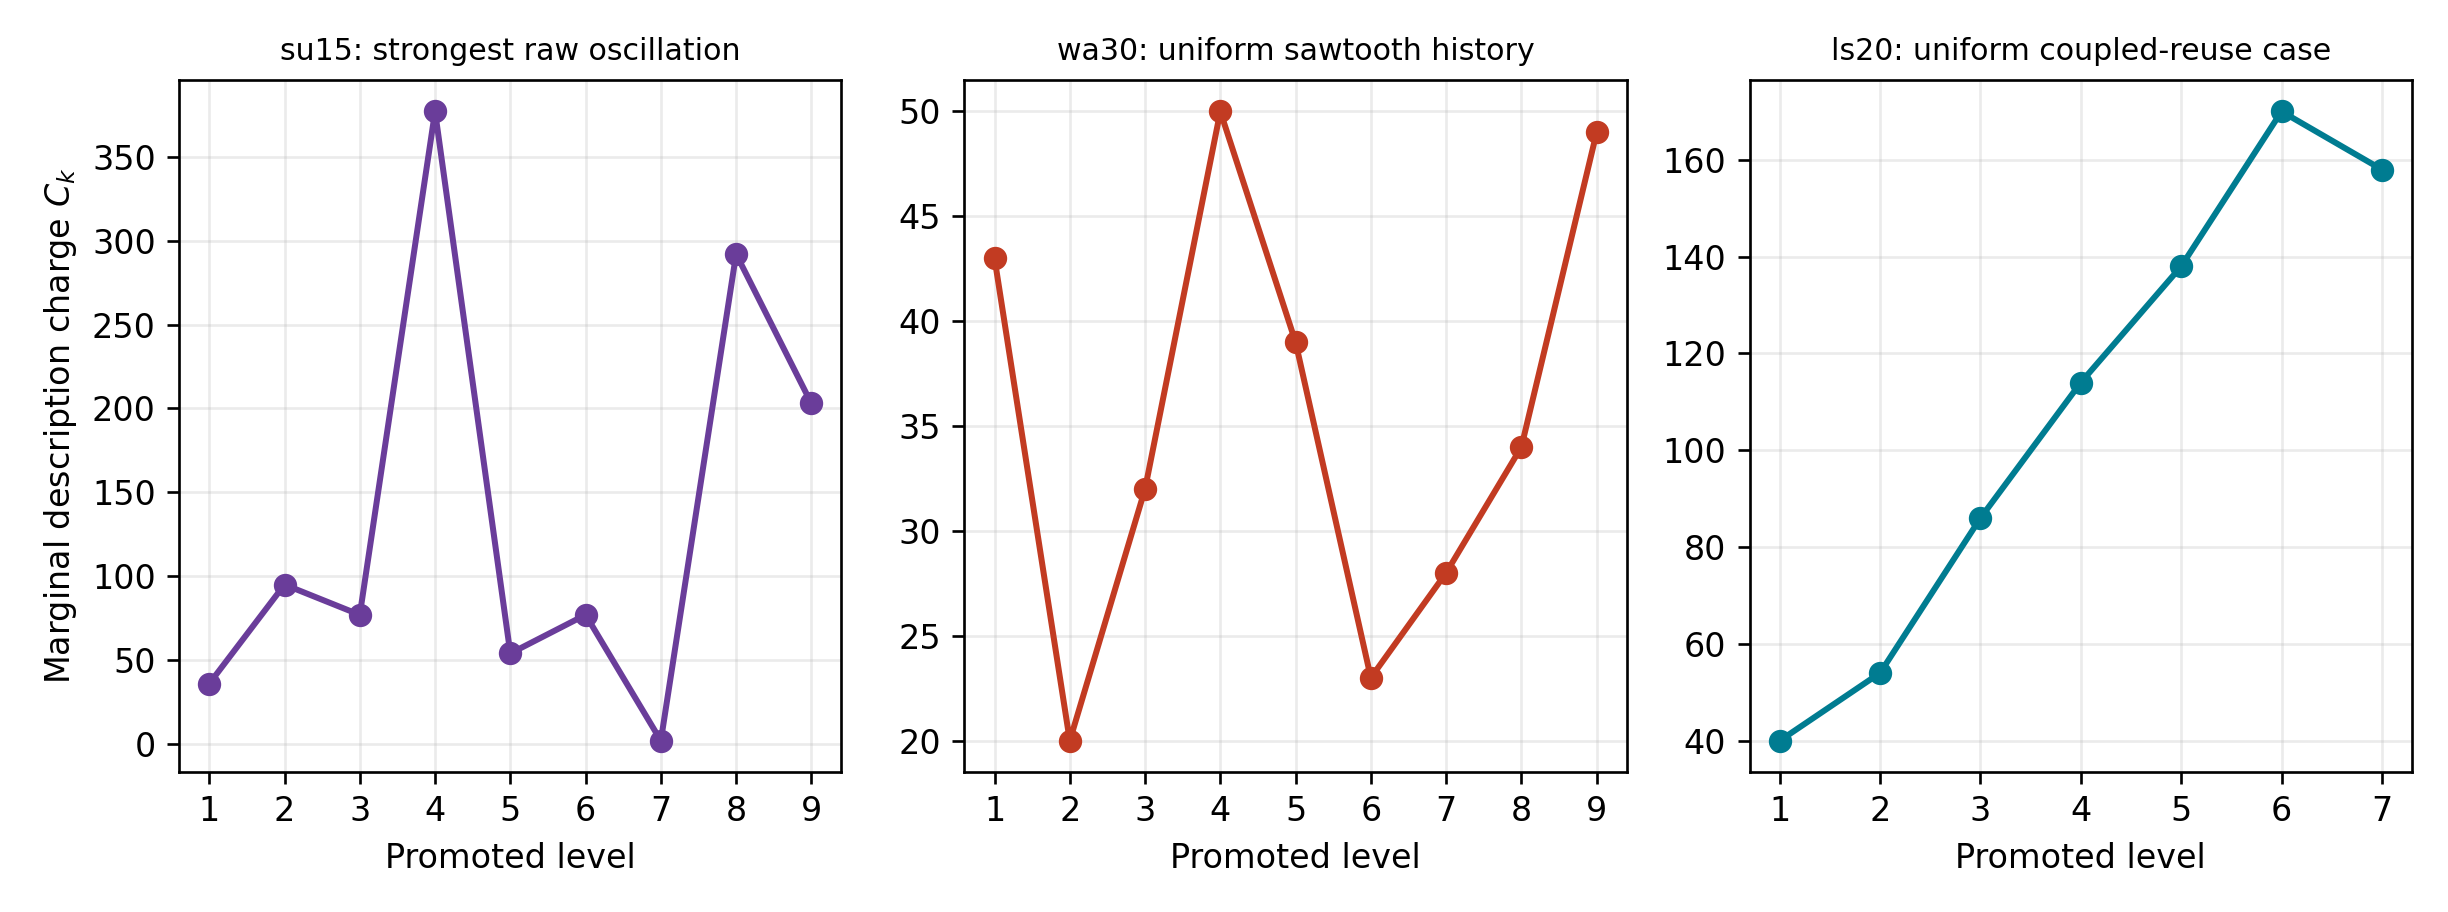
\includegraphics[width=0.98\textwidth]{figures/marginal_complexity_profiles.png}
\caption{Three checkpoint-recorded marginal profiles. \texttt{su15} has the strongest
raw oscillation (seven direction reversals in seven successive nonzero transitions),
but the scalar shape alone is not a reuse claim. \texttt{wa30} is the strongest
complete uniform-history sawtooth, while \texttt{ls20} supplies the source-coupled
unchanged-leg witness discussed in the text.}
\label{fig:marginal-profiles}
\end{figure}

\subsection{Interpretation of the complete histories}
The two uniform games give complementary profiles. In \texttt{ls20}, the
harness-native charge rises through L6 because each compact route contributes retained
literal information, then decreases slightly at L7. The exact conditional-AST measure
answers a different question: it falls sharply at L2 while the winning player directly
calls the unchanged \texttt{follow\_cardinal\_runs} leg. In \texttt{wa30}, the
harness-native ledger alternates three times, but its adjacent entry points call newly
named level-specific routines; it is therefore a complete measured sawtooth without a
strict coupled direct-call witness. A downward marginal trend is not expected in
general: the profile can fall when an empirical policy colimit extends cheaply and rise
when compatibility conditions or retained plan information change.

Across all checkpoint ledgers, \texttt{su15} is the most visibly oscillatory profile.
It is retained in Fig.~\ref{fig:marginal-profiles} as a descriptive scalar example, not
promoted to the main source-coupled case study: the frozen score release certifies its
endpoint paths, while the manuscript does not preserve a uniform exact acquisition-
source sidecar for every \texttt{su15} level. This distinction prevents post-hoc source
reconstruction from being mistaken for historical complexity dynamics.

\subsection{Bounded cross-game campaign}
To test whether the complete solves depended on per-game architecture, we applied the
same universal producer and promotion protocol across the suite. The resulting learned
programs are game- and level-dependent, but their production contract is unchanged.
The frozen release promotes at least one boundary in every game, completes 24 games,
and reaches \texttt{lf52} 8/10. Figure~\ref{fig:bounded-profiles} retains the five
multi-level profiles from the first portability experiment, now extended to their
frozen frontiers on a common scale. These profiles place low net-growth transitions
beside larger retained changes rather than enforcing monotone decline.

The receipt-bound payload passed local taint, action-protocol, source replay, path
replay, hash, and manifest checks, a full 25-game ONLINE shakedown, and the definitive
\href{https://arcprize.org/scorecards/cf75e14b-2c25-41cb-bc70-53bd57411edb}{official
Competition-Mode replay}. Failed attempts remain outside the release tree. Thus the
two-level remainder is resource-truncated, not a proof of an architectural ceiling. The
compute-completeness theorem in Section~\ref{sec:compute} supplies the algorithmic
statement behind this reading: whenever a finite replay-valid continuation exists in
the proposal language and the search schedule is fair, continuing search finds it in
finite enumerative time, or almost surely under a stagewise lower-bounded full-support proposer. The
unmeasured quantity is the practical rate---the distribution of the waiting time---not
the existence of the continuation under those conditions.

The reset-window allocation also tests whether stronger reasoning reduces the allowance
cost of finding compact continuations. Table~\ref{tab:effort-economics} charges failed
proposal turns to the effort that produced them and separates cold first-level
acquisition from continuation of a retained solver.
\begin{table}[H]
\centering
\small
\begin{tabular}{@{}llrrrr@{}}
\toprule
Phase & Effort & Attempts & Clears & Displayed points & Points/clear \\
\midrule
Cold L1 & medium & 4 & 3 & 4 & 1.333 \\
Cold L1 & high & 15 & 12 & 18 & 1.500 \\
Continuation L2+ & medium & 23 & 7 & 39 & 5.571 \\
Continuation L2+ & high & 7 & 1 & 14 & 14.000 \\
\bottomrule
\end{tabular}
\caption{Descriptive reset-window allowance accounting. Integer-valued displayed
weekly percentage is the hard cost coordinate because timed-out streams may omit final
token usage. High continuation attempts are selected after medium failures and are
therefore a harder, non-randomized cohort; the table is not a causal effort comparison.}
\label{tab:effort-economics}
\end{table}
High reasoning was effective for cold entry and eventually cleared \texttt{re86} L4
for two displayed points, but the window does not show a general high-effort compression
advantage. All four new literal-reuse wins, including the sharp coupled transitions
\texttt{ar25} L2 and \texttt{m0r0} L2, were produced by medium turns. The appropriate
operational conclusion is consequently phase- and frontier-specific: use medium for
first continuation search, retain clean WIP, and reserve high for a bounded escalation
rather than treating it as intrinsically cheaper. Under this sequential policy, the
decision-relevant future statistic is the incremental high-effort rescue rate after a
clean medium failure, with all failed and successful allowance charges retained in the
denominator; pooled effort averages remain confounded by frontier difficulty. A
retrospective application of that rule finds one replay-validated rescue in six
qualifying high turns, charged 12 displayed points in total. This $1/6$ observation
is too small and adaptively selected to estimate an intrinsic effort effect, but it
does show why high should remain a bounded fallback rather than the default.

\begin{figure}[t]
\centering
% Generated by scripts/generate_figures.py
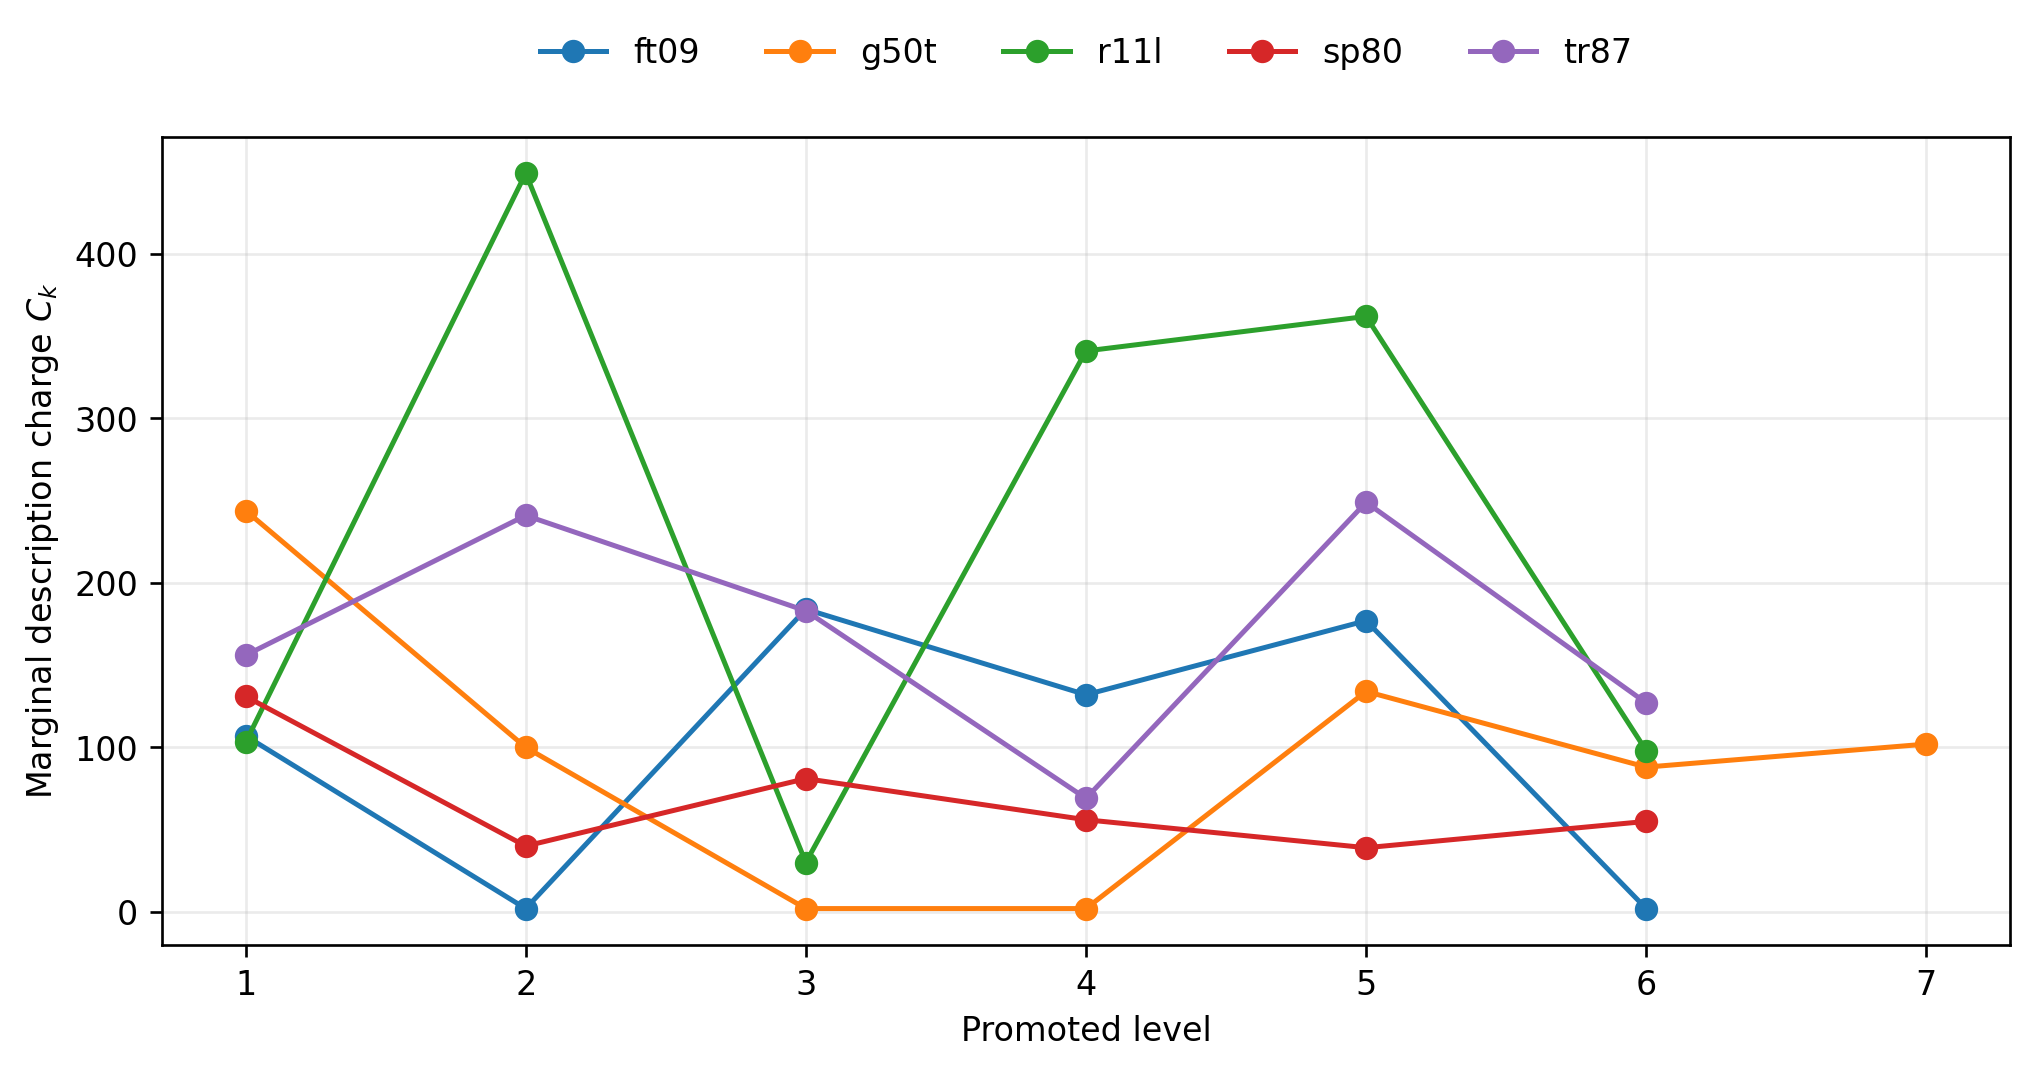
\includegraphics[width=0.92\textwidth]{figures/bounded_campaign_profiles.png}
\caption{Marginal profiles for the five bounded runs, read directly from frozen
checkpoints. Curves end at each verified frontier (levels 6--7). A shared ordinate preserves cross-game
magnitude. Low points measure small positive net source growth; they constitute reuse
evidence only where the corresponding player invokes previously charged routines and
fresh replay succeeds.}
\label{fig:bounded-profiles}
\end{figure}

This interpretation yields two testable predictions for future, prospectively logged
runs. Repeated layout variants under stable mechanics should produce low marginal
increments after the first successful abstraction. A mechanic change should produce an
increment whose source diff localizes to new state representation, control, or glue,
provided offsetting deletions do not hide it under Eq.~\eqref{eq:marginal-c}. A scalar
score makes neither prediction inspectable; the promoted transition history does.

% Generated by scripts/reproduce_manuscript.py; do not edit.
\newcommand{\GKMRetainedCheckpoints}{180}
\newcommand{\GKMExactWins}{180}
\newcommand{\GKMExactAdjacent}{154}
\newcommand{\GKMMemoryTransitions}{0}
\newcommand{\GKMComparable}{153}
\newcommand{\GKMDecreases}{70}
\newcommand{\GKMSharpDrops}{23}
\newcommand{\GKMHardReuse}{57}
\newcommand{\GKMCoupledWitnesses}{14}
\newcommand{\GKMUncoupledSharp}{9}
\newcommand{\OPINERetainedCheckpoints}{146}
\newcommand{\OPINEExactWins}{146}
\newcommand{\OPINEExactAdjacent}{121}
\newcommand{\OPINEMemoryTransitions}{0}
\newcommand{\OPINEComparable}{115}
\newcommand{\OPINEDecreases}{49}
\newcommand{\OPINESharpDrops}{14}
\newcommand{\OPINEHardReuse}{4}
\newcommand{\OPINECoupledWitnesses}{2}
\newcommand{\OPINEUncoupledSharp}{12}
\newcommand{\OPINETraceSolveEvents}{153}
\newcommand{\OPINEAnalyzerOrUnknownWins}{142}
\newcommand{\BaselineOneRetainedCheckpoints}{160}
\newcommand{\BaselineOneExactWins}{50}
\newcommand{\BaselineOneExactAdjacent}{18}
\newcommand{\BaselineOneMemoryTransitions}{0}
\newcommand{\BaselineOneComparable}{8}
\newcommand{\BaselineOneDecreases}{5}
\newcommand{\BaselineOneSharpDrops}{0}
\newcommand{\BaselineOneHardReuse}{0}
\newcommand{\BaselineOneCoupledWitnesses}{0}
\newcommand{\BaselineOneUncoupledSharp}{0}
\newcommand{\BaselineOneReportedClears}{174}
\newcommand{\BaselineOneExactAuthoredContractions}{4}
\newcommand{\BaselineOneDirectLiteralWins}{4}
\newcommand{\BaselineOneInlineLiteralWins}{6}
\newcommand{\BaselineOneExecutorLiteralWins}{8}
\newcommand{\RetrodictRetainedCheckpoints}{170}
\newcommand{\RetrodictExactWins}{0}
\newcommand{\RetrodictExactAdjacent}{0}
\newcommand{\RetrodictMemoryTransitions}{145}
\newcommand{\RetrodictComparable}{0}
\newcommand{\RetrodictDecreases}{0}
\newcommand{\RetrodictSharpDrops}{0}
\newcommand{\RetrodictHardReuse}{0}
\newcommand{\RetrodictCoupledWitnesses}{0}
\newcommand{\RetrodictUncoupledSharp}{0}
\newcommand{\RetrodictMemoryContractions}{76}
\newcommand{\CoupledWitnessEnumeration}{GKM \texttt{ar25} L2, $622\!\to\!175$, calling unchanged \texttt{repeat\_action}; GKM \texttt{cn04} L2, $710\!\to\!337$, calling unchanged \texttt{rotate\_quarter\_turns}, and \texttt{walk}; GKM \texttt{g50t} L4, $2238\!\to\!168$, calling unchanged \texttt{solve\_unlock\_macro}; GKM \texttt{ka59} L2, $810\!\to\!301$, calling unchanged \texttt{move\_steps}, and \texttt{select\_at}; GKM \texttt{lf52} L3, $1602\!\to\!157$, calling unchanged \texttt{solve\_peg\_solitaire\_with\_carrier}; GKM \texttt{lp85} L2, $698\!\to\!189$, calling unchanged \texttt{repeat\_click}; GKM \texttt{ls20} L2, $737\!\to\!247$, calling unchanged \texttt{follow\_cardinal\_runs}; GKM \texttt{m0r0} L2, $673\!\to\!265$, calling unchanged \texttt{follow\_action\_sequence}; GKM \texttt{sb26} L3, $1796\!\to\!158$, calling unchanged \texttt{copy\_visible\_color\_code\_into\_diagram}; GKM \texttt{sc25} L2, $1131\!\to\!279$, calling unchanged \texttt{move\_until\_level\_progress}, and \texttt{select\_grid\_cells\_of\_color}; GKM \texttt{sp80} L5, $2011\!\to\!486$, calling unchanged \texttt{drive\_objects}; GKM \texttt{su15} L7, $1246\!\to\!161$, calling unchanged \texttt{merge\_equal\_squares\_around\_moving\_cutter}; GKM \texttt{tu93} L5, $1302\!\to\!186$, calling unchanged \texttt{drive\_dynamic\_maze\_via\_color}; GKM \texttt{tu93} L7, $1440\!\to\!212$, calling unchanged \texttt{drive\_dynamic\_directional\_waypoints}; OPINE \texttt{lp85} L4, $5818\!\to\!2550$, calling unchanged \texttt{\_cross\_components}, \texttt{\_cursor\_pairs}, and \texttt{\_square\_blocks}; OPINE \texttt{tu93} L3, $7091\!\to\!2608$, calling unchanged \texttt{\_find\_player}, \texttt{\_goal\_topleft}, and \texttt{transition\_function}}

\section{Artifact-Level Comparison}
\subsection{Contemporary ARC-AGI-3 systems}
ARC Prize separates verified model evaluation from the public community track for
domain-specific harnesses. Public-track scores are self-reported by default; a server
scorecard validates submitted action replay, but does not by itself audit what
information produced the policy. The Foundation therefore cautions against treating a
public harness score as a held-out generalization result~\cite{arcagi3,arcprize2026policy}.
We consequently compare performance, replay, epistemic provenance, and solver-growth
evidence as distinct claims.

The graph-exploration baseline belongs to the six-game preview generation, not the
current 25-game public set. It officially solved 12 of 25 private preview levels; after
the authors corrected a disclosed reset-handling bug, five private reruns ranged from
14 to 19, with median 17. At the paper's 4{,}000-interaction comparison point it solves
two \texttt{ls20} levels and reports that levels~3+ become intractable for exhaustive
exploration~\cite{arcagi3graph}. It is a useful historical private-set baseline, but
its non-learning within-level graph is not a cross-level executable skill trajectory.

The original executable-world-model study reports \texttt{ls20} 7/7 with both tested
models and \texttt{wa30} 7/9 versus 4/9 depending on the model
\cite{arcagi3worldmodels}. Its follow-up v1.6 verification agent, using
GPT-5.6-sol, reports all 183 public levels solved at both xHigh and max effort, with
98.97 and 98.77 RHAE respectively; its textual agent also solves 183/183 at max
\cite{rodionov2026ablations}. The authors explicitly call this public-set saturation:
the model postdates the public games, visual recognition remains a contamination
possibility, and no semi-private or fully private result is reported. They also disclose
and exclude earlier development runs in which agents recovered the true game ID, used
web search, or opened a second unscored client. The current paper documents Docker
isolation, hidden identifiers, restricted service egress, and a published checksummed
run archive. This is materially stronger provenance evidence than a score alone, but
the latest archive has not yet been reduced to exact solve-boundary description
marginals.

OPINE-World reports 20/25 games, 160/183 levels, and 78.4 RHAE on one public run per
game~\cite{courtis2026opine}. Its reported frames-only Docker configuration excludes
the game source, and its paper reports a transcript audit for source, web, and credential
access. The released main logs reconstruct 153 positive-reward events rather than the
160-level headline without crossing into summary/report layers. Its frames-only
harness recomputes a Beta posterior over induced object-type/action consistency from
the cumulative cross-level replay buffer and exposes Thompson-ranked uncertain
dynamics to the analyzer. This Bayesian diagnostic guides exploration but does not
itself choose actions. The executable sawtooth claim is narrower: among
\OPINEComparable{} comparable adjacent engine marginals, \OPINEDecreases{} decrease
and \OPINESharpDrops{} decrease by at least one half, but the
\OPINEUncoupledSharp{} uncoupled sharp drops accompany transient analyzer wins whose
executable policies were not retained. Only \OPINECoupledWitnesses{} sharp drops are
coupled to a synthesized winning planner that
directly invokes unchanged earlier engine definitions: \texttt{lp85} level~4
and \texttt{tu93} level~3. OPINE therefore has extensive cross-level data and hypothesis reuse,
but only these two released boundaries certify the narrower
Kolmogorov--Schmidhuber executable path.

\subsection{Solved checkpoints as the common unit}
We also examined the released artifacts of OPINE-World~\cite{courtis2026opine},
the GPT-5.5 xHigh \texttt{baseline1} run~\cite{arcagi3worldmodels}, and the
Retrodict v1 artifact set~\cite{brown2026retrodict}. The comparison uses one rule
throughout: the
checkpoint for level $L$ is the program or memory state present when $L$ was actually
cleared. A later retained snapshot is equivalent only if no measured component changed
after the winning action. Interim synthesis rounds, repeated same-level Git commits,
and within-level notebook edits are excluded. This rule prevents both ordinary search
churn and post-win cleanup from being misreported as a solver sawtooth.

Four quantities must then remain separate. The cumulative executable coordinate
$D(S_L)$ measures the retained solver at the $L$th clear. The conditional acquisition
cost measures what was added since $S_{L-1}$. An operational reuse witness shows that
the later clear actually invoked an unchanged earlier component. Finally, notebook,
transcript, and context length describe agent memory, not executable solver complexity.
Compression of one quantity does not imply compression of the others. Retained
observations, posterior counts, notes, transcripts, and proposer/action trajectories
are admissible broad reuse, but do not alone establish an executable solver sawtooth.

To compare conditional novelty without treating same-size replacement as free, let
$A(P_L)$ be the multiset of normalized top-level AST statements in the exact winning
program $P_L$. We use
\begin{equation}
 M_L =
 \left|\operatorname{zlib}_9\!\left(
 A(P_L)\setminus_{\mathrm{multi}} A(P_{L-1})\right)\right|,
 \label{eq:conditional-ast}
\end{equation}
where the multiset difference removes only literal normalized-AST matches and the
remaining statements are serialized canonically. Thus unchanged source is available
as a dictionary, while a same-size rewrite is charged. We call $M_L\leq M_{L-1}/2$ a
sharp marginal drop. A drop is attributed to reuse only if the winning entry point
directly calls a named definition whose normalized AST is identical in $P_{L-1}$.
Equation~\eqref{eq:conditional-ast} is a computable conditional-description upper
bound, not machine-independent Kolmogorov complexity; its values are compared only
within an artifact lineage. Thus the narrow Kolmogorov--Schmidhuber witness requires
four things at once: exact adjacent winning executable states, a conditional
description relative to the preceding win, a sharp reduction, and an actual call from
the later winning entry point into unchanged preceding-win machinery. A direct call
without a sharp drop is hard executable reuse, but not a coupled sawtooth witness.

The result is asymmetric. OPINE-World has hard level-to-level reuse under the exact
winning-entry-point test; the audited GPT-5.5 \texttt{baseline1} lineage does not, and
the Retrodict v1 artifact set does not release the executable checkpoints needed to
pass it. These statements do not impute the same solve-boundary result to baseline1
v1.6 or Retrodict v2. GKM supplies the strongest literal-leg evidence in the measured
exact set. This source denominator is narrower than GKM's endpoint result: all 181
claimed levels are replay-verified wins, while the pinned winning-source audit admits
174 exact checkpoints. It excludes \texttt{ft09} L2 and \texttt{tr87} L1--L6 because
their endpoint capsules are replay-valid deterministic path reconstructions rather than
admissible winning-source checkpoints for source-marginal comparison.

\begin{table}[H]
\centering
\scriptsize
\begin{tabularx}{\textwidth}{@{}l>{\raggedright\arraybackslash}p{0.19\textwidth}
  >{\raggedright\arraybackslash}p{0.24\textwidth}
  >{\raggedright\arraybackslash}X@{}}
\toprule
System & Replay/source boundary coverage & Conditional AST marginal &
Direct literal reuse at the win \\
\midrule
GKM & 181/183 replay-verified level wins; \GKMExactWins{} exact winning-source
checkpoints admitted by audit and \GKMExactAdjacent{} adjacent source transitions &
\GKMDecreases{} decreases among \GKMComparable{} comparable marginals;
\GKMSharpDrops{} sharp drops &
\GKMHardReuse{} winning players directly call unchanged legs;
\GKMCoupledWitnesses{} are sharp coupled witnesses \\
OPINE-World & \OPINEExactWins{} pre-solve engines for
\OPINETraceSolveEvents{} positive-reward trace
events; \OPINEExactAdjacent{} adjacent transitions &
\OPINEDecreases{} decreases among \OPINEComparable{} comparable marginals;
\OPINESharpDrops{} sharp drops &
\OPINEHardReuse{} synthesized-planner wins directly call unchanged engine definitions.
Sharp coupled
witnesses: \texttt{lp85} L4 and \texttt{tu93} L3 \\
\texttt{baseline1} & \BaselineOneRetainedCheckpoints{} post-solve snapshots for
\BaselineOneReportedClears{} clears; \BaselineOneExactWins{} exact winning sources and
\BaselineOneExactAdjacent{} exact adjacent transitions &
\BaselineOneDecreases{} decreases among \BaselineOneComparable{} comparable
marginals; \BaselineOneSharpDrops{} sharp drops &
\BaselineOneHardReuse{}. The \BaselineOneExactAdjacent{} winning commands are fresh
action programs: \BaselineOneDirectLiteralWins{} direct actions,
\BaselineOneInlineLiteralWins{} inline plans, and
\BaselineOneExecutorLiteralWins{} plans passed to \texttt{plan\_executor.py} \\
Retrodict v1 & \RetrodictRetainedCheckpoints{} solved memory checkpoints;
\RetrodictMemoryTransitions{} memory transitions; \RetrodictExactWins{} exact
executable winning checkpoints &
\RetrodictMemoryContractions{} memory contractions, but
\RetrodictExactAdjacent{} executable adjacent and \RetrodictComparable{} comparable
marginals &
\RetrodictHardReuse{} executable witnesses: released checkpoints contain playbook
memory, not winning entry points \\
\bottomrule
\end{tabularx}
\caption{Source-auditable solved-checkpoint comparison. A marginal comparison $M_L$ versus
$M_{L-1}$ requires the corresponding consecutive exact winning sources. A literal
reuse witness requires a direct call from the winning entry point; retained but
uninvoked definitions do not qualify. Counts describe historical source-audit coverage,
not replay-verified level coverage or performance.}
\label{tab:audit-axes}
\end{table}

\paragraph{Sharp coupled witnesses.}
\begingroup\footnotesize\sloppy
Exactly \GKMCoupledWitnesses{} GKM and \OPINECoupledWitnesses{} OPINE
transitions satisfy both the sharp-drop and literal-call tests:
\CoupledWitnessEnumeration. The rows in Table~\ref{tab:audit-axes} report marginal
screens and literal reuse separately so that a contraction alone cannot be promoted
to a transfer claim.
\endgroup

\subsection{What the comparator artifacts establish}
The \OPINETraceSolveEvents{} positive-reward events are the coverage of the released
main traces, not a
recalculation of OPINE's reported 160-level result: \texttt{s5i5} lacks a summary,
\texttt{sb26} has a repaired summary with one more reward than its main log, and
\texttt{tr87} has the converse mismatch. We report these gaps rather than impute
solve-boundary programs.
Only \OPINEHardReuse{} measured positive-reward traces were emitted by the synthesized
planner:
\texttt{lp85} levels~3, 4, and~6 and \texttt{tu93} level~3. All
\OPINEHardReuse{} directly call
engine definitions that are literal matches to the preceding winning checkpoint.
\OPINECoupledWitnesses{} are sharp marginal drops. At \texttt{lp85} level~4, the normalized
\texttt{planner} itself is identical to the level-3 winner and directly calls unchanged
\texttt{\_cross\_components}, \texttt{\_cursor\_pairs}, and
\texttt{\_square\_blocks}. At
\texttt{tu93} level~3, the winning planner directly calls unchanged
\texttt{\_find\_player}, \texttt{\_goal\_topleft}, and
\texttt{transition\_function}. These are executable
world-model reuse, not merely retention.

The other \OPINEAnalyzerOrUnknownWins{} analyzer/unknown wins include the
\OPINEUncoupledSharp{} uncoupled sharp OPINE drops. The retained
\texttt{game\_engine.py} can contract or remain identical while the transient winning
policy changes; \texttt{tr87} level~6 and \texttt{tu93} level~8 have zero retained
engine novelty but no released executable analyzer entry point. Those cases are not
counted as literal solver reuse. The \OPINEHardReuse{} synthesized-planner witnesses
nevertheless falsify the categorical claim that OPINE solves every level wholly anew.
\OPINEHardReuse{} of \OPINEExactAdjacent{} is
a lower bound under the deliberately narrow retained-entry-point test, not an estimate
of total operational reuse: OPINE's cumulative replay, analyzer session and notes,
shared hypotheses, and normally inherited engine all cross level boundaries. The
reported configuration leaves autonomous planning off, however, and the analyzer's
use of its model-backed planner tool is conditional. Because the transient winning
analyzer entry points were not retained, the audit neither credits nor denies their
causal dependence on those priors.

The \texttt{baseline1} result requires a finer timing distinction. Its Git snapshot is
taken only at the start of the next agent iteration. The level-completion prompt asks
the agent to stop real actions but permits it to prepare deliverables, including
further Python edits, before that snapshot. Retained-source contractions between
adjacent post-solve states are therefore only a diagnostic denominator. We aligned
all \BaselineOneReportedClears{} real clears to client or guarded-executor output and
then inspected file changes through the end of each winning Codex turn.
\BaselineOneExactWins{} of the \BaselineOneRetainedCheckpoints{} retained snapshots
have no post-win Python edit; only \BaselineOneExactAdjacent{} adjacent transitions
have exact endpoints on both sides. \BaselineOneExactAuthoredContractions{} strict
authored-source contractions survive, and all also contract after AST normalization.

They are retained-artifact contractions, not demonstrated solver reuse. Across all
\BaselineOneExactAdjacent{}
exact adjacent transitions, the command that produces the real clear invokes no
retained world-model definition. \BaselineOneDirectLiteralWins{} are direct action
commands, \BaselineOneInlineLiteralWins{} contain inline literal plans, and
\BaselineOneExecutorLiteralWins{} pass literal plans to the generic
\texttt{plan\_executor.py}. The four contracting workspaces retain 18--23 unchanged
core definitions, but uninvoked code is not part of the winning entry point. The
conditional AST marginal decreases in five of the eight transitions for which
successive marginals can be compared; none decreases by half. The baseline1 artifacts
therefore supply no coupled marginal-drop/literal-reuse witness under this test.

The Retrodict v1 artifacts demonstrate a third phenomenon. Their traces reconstruct
curated memory at every solve boundary, and that memory repeatedly expands and
contracts as the playbook is rewritten. Nearly all selected runs retain no
substantive scratch Python at any solve checkpoint; the exceptions,
\texttt{cn04} and \texttt{r11l}, show scratch expansion but no scratch contraction.
Thus that release supports memory reuse across context resets, not a
Kolmogorov proxy for an executable solver trajectory. Retrodict v2 also deliberately
reuses observations, action trajectories, and a playbook, so the categorical claim
that it has no reuse would be false. Those are admissible experience reuse, but the
release does not expose a per-level executable winning entry point from which to
measure a coupled conditional-description sawtooth. Log length, action count, and
provider context are not substitutes.

\paragraph{Relation to the Kolmogorov--Schmidhuber thesis.}
The hard result is not an architectural slogan. The G\"odel--Kolmogorov Machine has
\GKMHardReuse{} exact wins whose players directly call unchanged leg literals.
\GKMCoupledWitnesses{} coincide with sharp marginal drops and are enumerated above.
The other \GKMUncoupledSharp{} sharp GKM drops lack an unchanged direct leg call and are not labeled
reuse. A non-sharp witness occurs at \texttt{ft09}
level~6: its winning player directly calls the unchanged
\texttt{solve\_coupled\_key\_board} acquired at level~5 with a non-sharp decrease in
$M_L$. The historical net-growth ledger is not substituted for the conditional AST marginal.
This joint test is stronger than either a size curve or a static library count.

GKM remains the closest architectural fit to the present Kolmogorov--Schmidhuber
selection thesis because it attempts incumbent-leg execution before invention, requires
strict replay progress for promotion, and exposes marginal description cost as the
free energy coordinate governing candidate comparison, debrief, and the forward
selection program. Its cumulative winning source
still expands at every exact adjacent transition. OPINE is a genuine counterexample to
the stronger exclusivity claim: it has \OPINEHardReuse{} direct literal
engine-reuse wins and \OPINECoupledWitnesses{} sharp coupled drops. The audited
GPT-5.5 baseline1 lineage has no such
winning-entry-point witness in the exact set, and Retrodict v1 exposes memory rather
than executable solver checkpoints. Failing to cite Kolmogorov or Schmidhuber is not
itself a defect: the operational questions are whether acquisition cost is measured and
whether later wins actually invoke retained earlier structure.

The analyzers and machine-readable rows are produced by:
\begin{quote}\small
\path{arc/audit_gkm_solved_checkpoints.py}\\
\path{arc/audit_baseline1_artifacts.py}\\
\path{arc/audit_opine_solved_checkpoints.py}\\
\path{arc/audit_retrodict_artifacts.py}\\
\path{arc/audit_marginal_literal_reuse.py}
\end{quote}
They preserve source and normalized-AST measures separately, record winning-policy
provenance, and never substitute an interim revision for a solve checkpoint. The
semiautomated reproduction entry point is
\path{arc/manuscript/scripts/reproduce_manuscript.py}; it recomputes the local GKM
rows, checksum-pins or rebuilds comparator rows, regenerates the figures and
\path{generated/comparator_stats.tex}, runs the audit/figure tests, and can rebuild
the PDF. Its latest machine-readable report is
\path{arc/manuscript/reproduction_report.json}.


\section{Discussion}
\label{sec:discussion}
\subsection{What the artifacts establish}
The campaign demonstrates the intended solver-growth dynamics. New mechanics enter as
new executable cells, recurring mechanics can be reached through thin attaching maps,
and some later wins have sharply smaller conditional source novelty. The exact winning-
checkpoint audit identifies \GKMHardReuse{} GKM transitions whose players directly
call unchanged leg definitions. \GKMCoupledWitnesses{} also exhibit sharp
conditional-AST contractions, as enumerated in the artifact comparison. These are the
empirical form of
Eq.~\eqref{eq:cone-marginal}: the old cell remains in the colimit and the new promotion
pays mainly for the binding.

The complete \texttt{wa30} and \texttt{ls20} histories occupy different regions of the
structure function. \texttt{ls20} reuses one unchanged execution leg at every level;
its exact conditional-AST novelty falls sharply at L2 even though the harness-native
ledger later rises with retained route information. \texttt{wa30} has a complete
alternating harness-native profile but no strict adjacent direct-call witness under the
declared test. The free energy framework permits exactly this distinction: scalar
charge, source factorization, retained code length, and historical construction action
are different observables.

\subsection{Why the categorical language is load-bearing}
A Boolean inclusion lattice of observed traces cannot express what the LLM contributes.
The proposer does not merely select a larger set of state--action pairs. It invents an
object $B_k$, chooses a boundary $A_k$, supplies a cofibration $A_k\hookrightarrow B_k$,
and constructs an attaching map into the incumbent. Those morphisms determine whether a
shared routine can be rebound, whether two components agree on an overlap, and whether
the resulting player factors through the existing library. The universal property of
the pushout then states what it means for the composed solver to be the least gluing of
those data.

Likewise, the pointwise Kan-extension view separates two sources of generalization. The
colimit performs the gluing; the comma-category morphisms encode the inductive bias. A
failure to transfer often means that the repository lacks the right slot, predicate,
scene relation, or connector morphism. The LLM's scientific role is to enrich that
morphism vocabulary and propose the missing attachment. Replay is the empirical test of
whether the proposed semantic triangles commute on the admitted histories.

\subsection{The force of the compute claim}
The resource records and the completeness theorem answer different questions. The
records show that the reported partial campaigns ended at imposed caps, interruptions,
or exhausted credits rather than at a preserved proof of impossibility. The theorem
shows that, for any finite replay-valid continuation expressible in the proposal
language, fair continued search reaches it. Since literal finite plans are expressible,
every finitely solvable deterministic instance has such a continuation, and a finite
suite of such instances is completed after finite enumerative computation. The title's
``compute-bounded'' qualifier therefore does not retract the solving claim; it identifies
the independent variable governing how far the monotone archive has advanced.

What remains empirical is the rate. The probabilities $p_k$, the benefit of inherited
legs, the effect of proposer strength, and the shape of $V_B$ require prospective budget
curves. Recent ARC-AGI-3 ablations with stronger coding models and greater reasoning
effort independently report substantial gains from compute and a verification treatment
that solves the public set in the strongest tested setting~\cite{rodionov2026ablations}.
That result is not a compute-matched comparison with GKM, but it reinforces the broader
claim that model capability, search budget, and executable verification are first-order
variables rather than incidental implementation details.

\subsection{A forward program: curiosity, phase structure, and open-ended PowerPlay}
The current ARC histories are a first finite section of a larger program. Four
experiments follow directly from the theory.

First, prospectively preserve multiple valid candidates at each depth and sweep
$\lambda$. This estimates $C^*(r)$ instead of a single path and exposes the supported
regimes of Eq.~\eqref{eq:model-dual}. Second, sample proposal populations around each
$\lambda$ and track $\chi_C$; peaks predict transitions between literal plans, search
procedures, world models, and reusable leg compositions. Third, allocate controlled
proposal budgets to incumbents with and without inherited legs. The gap in the waiting-
time distributions estimates the computational value of the colimit library. Fourth,
replace the fixed level order by an archive-driven ecology that proposes probes and
microtasks with high expected free energy progress, implementing the curiosity signal in
Eq.~\eqref{eq:curiosity-progress}.

This program unifies the three historical ideas rather than placing them side by side.
The G\"odel-machine gate decides which self-rewrite becomes real. PowerPlay determines
that each rewrite must add a task or compress an old one without forgetting. Artificial
curiosity determines which experiment is worth performing next. Kolmogorov free energy
prices the structure, and inverse colimits state how the structure is assembled.

\subsection{Validity and scope}
The source coordinate is tied to a published representation, not invariant under all
program encodings. This is expected in the computable-proxy theory and motivates coding
sweeps rather than abandonment of complexity measurement. Deterministic path replay
certifies the admitted finite behavior, not robustness under arbitrary perturbations.
The taint detector blocks known private channels but is not a formal noninterference
proof. Historical proposer compute was not logged uniformly, so the current artifacts
cannot estimate the parameters in Eq.~\eqref{eq:completion-tail}. Finally, the semantic
image of a syntax pushout is tested on finite replay suites; a global behavior functor
need not preserve every colimit outside those suites.

These boundaries locate the next experiments without reducing the paper to an artifact-
existence statement. The contribution is a forward architecture with exact mathematical
structure, an asymptotic compute theorem, and executable instances in which the predicted
acquisition and reuse phenomena are visible.

\section{Conclusion}
The G\"odel--Kolmogorov Machine is a compute-bounded self-improving solver in the direct
lineage of G\"odel machines, PowerPlay, and artificial curiosity. Its generative step is
categorical: an LLM proposes executable legs together with interfaces, cofibrations, and
attaching morphisms. Its program step is an inverse colimit: the incumbent and an LLM-supplied cell are
glued by a pushout along an LLM-supplied cofibration and attaching map. Strictly additive
acquisitions form a sequential colimit, while debriefs are separated as replay-equivalent
refactors. Its verification step is an inverse system of first-passage depth certificates
that prevents capability forgetting without falsely requiring historical trace identity.
Its selection step is the free energy dual of a Kolmogorov structure function instantiated
by a computable source coordinate.

This combination supports a strong compute claim. A literal winning trace is a finite
cell, reusable abstractions are shorter cells with richer transfer, and a fair enumerator
or stagewise full-support proposer reaches any finite replay-valid attachment chain with enough
compute. The practical problem is therefore to reshape the waiting-time distribution:
use inherited colimits, free energy parsimony, PowerPlay's archive, and curiosity-driven
probes to find the right cell before brute force would.

The released campaign supplies ARC-AGI-3 evidence for this program. All 25 promoted
endpoints replay, covering 181 of 183 levels, and exact source-level witnesses show
unchanged legs participating in later wins with reduced marginal description, including
\GKMCoupledWitnesses{} sharp coupled GKM cases in the acquisition-history audit. The
definitive Competition card reports $98.11664037825032\%$; the distinct raw verified
coverage is $181/183=98.907103825137\%$, with 7001 stored path actions and 7069
official API calls. The uniform \texttt{wa30} and \texttt{ls20} histories give complete
ledgers of 318 and 760 respectively, each with one sequential promotion manifest per
level.
These distinctions strengthen rather than replace the central thesis. In the
compute-indexed sense proved here, any finite deterministic ARC-AGI-3 suite with finite
winning traces is solved by fair GKM search with literal-trace fallback; the released
campaign is a finite-budget prefix of that construction. The practical scientific
problem is to replace astronomical enumeration by reusable program growth, and the
mathematics of that growth is the mathematics of structure functions, inverse colimits,
cofibrations, and compute.

\paragraph{Acknowledgment.}
We thank OpenAI for providing access to GPT-5.6-sol.

\paragraph{Data availability statement.}
All data and code necessary for verification and reproducibility are contained in the GitHub repository \cite{gkmrepo}.

\paragraph{Author contribution and generative-AI disclosure.}
A.K. is the sole author of this manuscript and takes full responsibility for its
contents. Anthropic's Opus 4.8 and Fable 5 and OpenAI's GPT-5.6-sol were used as
text-to-text generative-AI tools during code development and manuscript preparation.

{\small
\bibliographystyle{plain}
\bibliography{references}
}
\end{document}
